\chapter{ATAS Experiments in Germanium}
\label{chap:ATAS_in_Ge}


\section{Introduction}







\begin{figure}
	\centering
	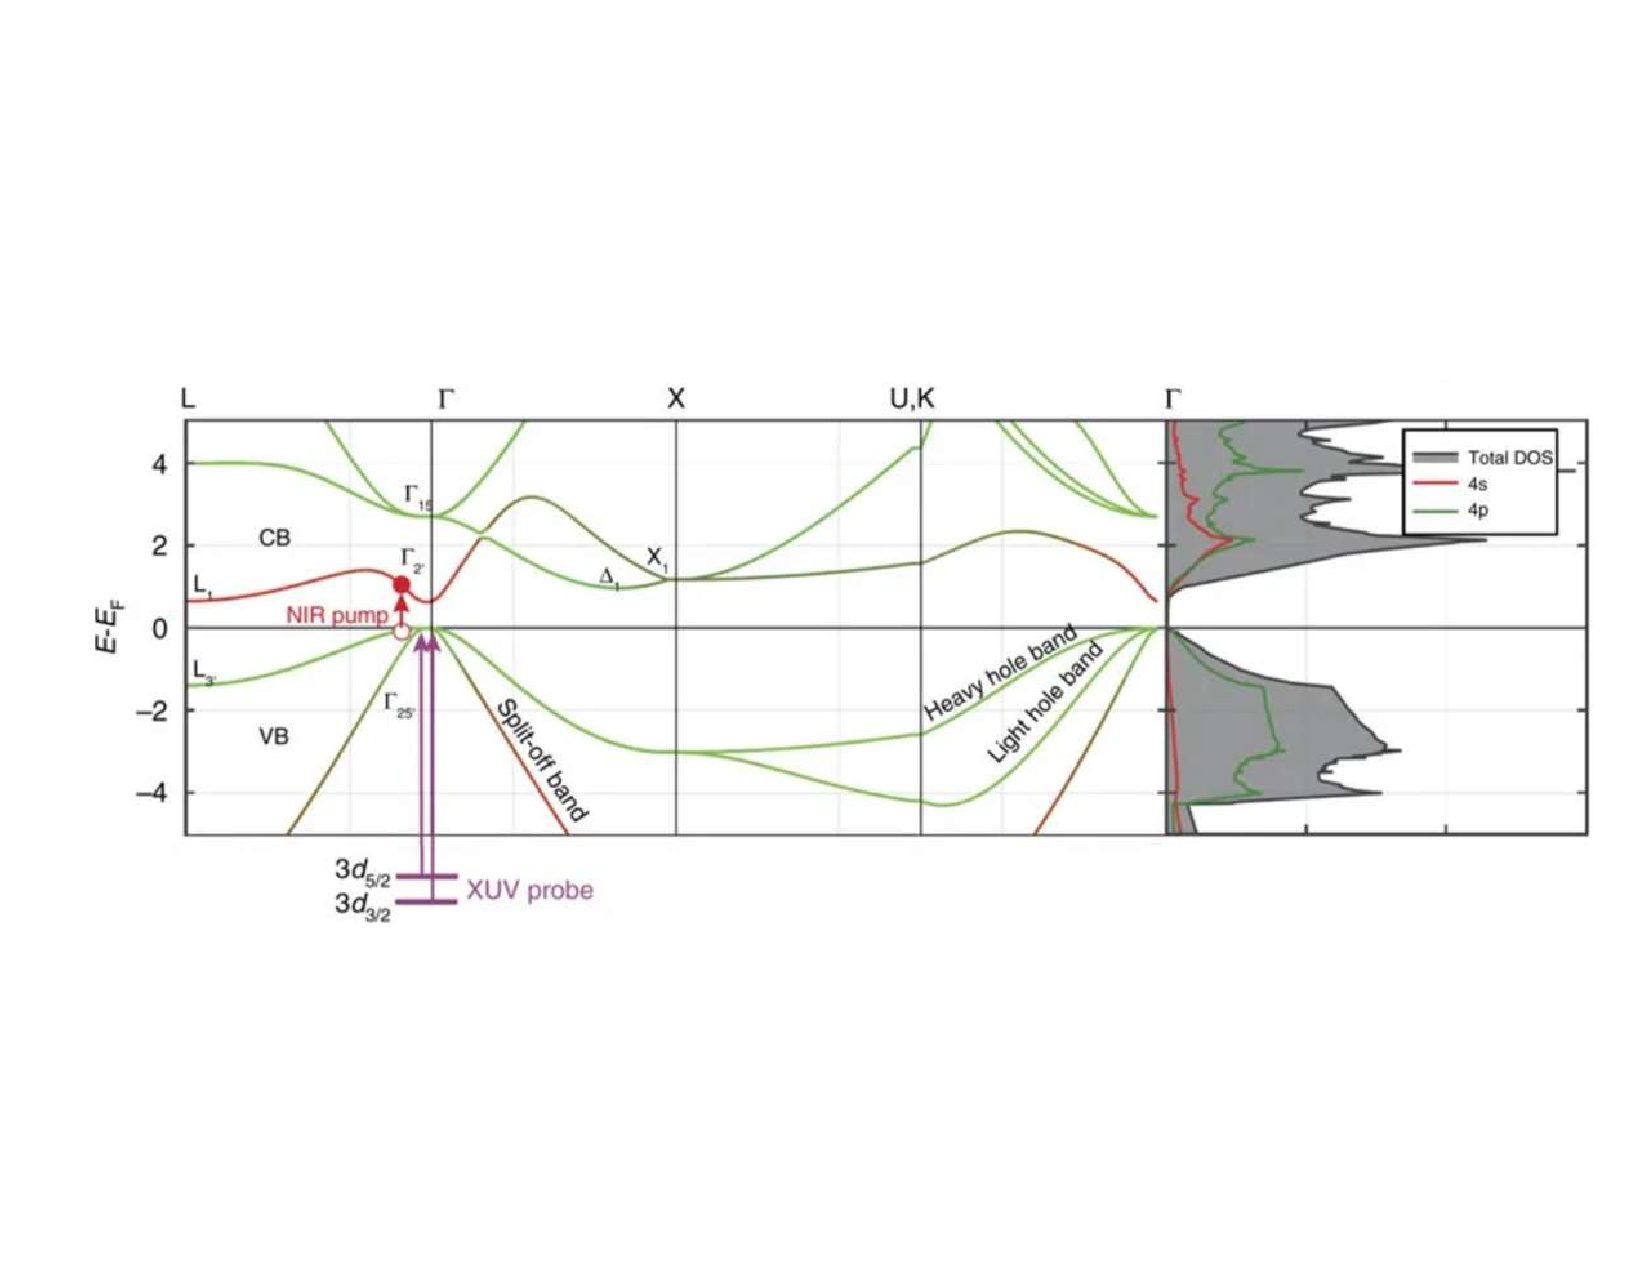
\includegraphics[width=0.75\textwidth]{figures/chap4/Ge_band_diagram_Zurch2017.pdf}
	\caption{Band structure and orbital character of germanium. Purple arrows indicate XUV-induced transitions from the $3d$ core levels to the valence bands. Red arrow indicates IR-induced transition across the direct band gap. Figure adapted from \cite{zurchDirectSimultaneousObservation2017}.}
	\label{fig:Ge_band_diagram}
\end{figure}

previous chapters: designed, built and tested a high-brightness XUV light source. haven't yet talked about the interferometer much? now, need to introduce the following concepts:
\begin{itemize}
	\item scientific motivation / goal for studying ATAS in condensed matter in general.
	\item general sample requirements (thickness, absorption edge)
	\item ground state measurements of various materials
	\item scientific motivation / goal for studying ATAS in germanium specifically.
	\item intensity / ionization inside germanium (TMM/Keldysh)
	\item experimental results of Ge ATAS

\end{itemize}

\section{Experimental Considerations}

\subsection{Sample Requirements}

\begin{figure}
	\centering
	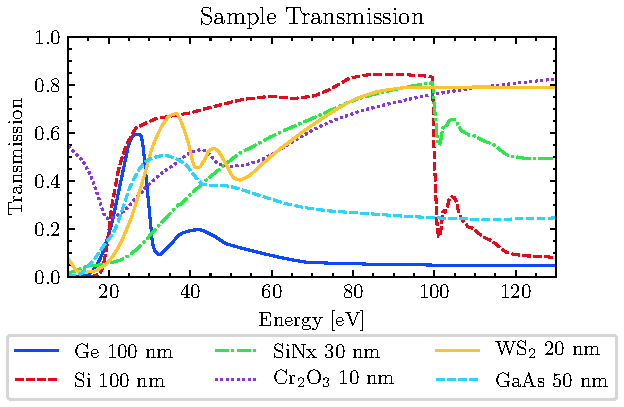
\includegraphics[width=0.75\textwidth]{figures/chap4/Sample_transmission_CXRO.pdf}
	\caption{Calculated XUV transmission of various materials. Data from \cite{gulliksonCXROXRayInteractions}.}
	\label{fig:Sample_trans_CXRO}
	% figure generated using \PythonScripts\CXRO\test\CXRO.py
\end{figure}

There are several sample requirements for a successful condensed matter transient absorption experiment. First and foremost, the sample needs to have an absorption edge within the bandwidth of the XUV source. Second, the material must be the correct thickness for a transmission measurement, given the capabilities of the XUV light source and detector. If the material is too thick, the ground state will absorb most of the XUV flux and the recorded spectrum will be too close to the noise floor of the apparatus. If it is too thin, insufficient XUV absorption will occur and the laser-induced change of the ground state (on the order of $1-10\%$) will be lost in the noise floor. As a general guideline, a sample that absorbs 50\% at the spectral feature of interest provides a good compromise between these conflicting requirements. \cref{fig:Sample_trans_CXRO} shows the expected transmission of several materials, calculated from the atomic scattering factors \cite{gulliksonCXROXRayInteractions}. We can see that a typical sample will be on the order of 10 - 200 nm thick, depending on the material.

Another upper bound for sample thickness comes from material dispersion. In any material, the XUV light ($n_{\text{XUV}} \sim 1$) will outpace the IR light ($n_{\text{IR}} > 1$). This effect can be significant even for ultrathin films. In order to keep the phase slippage between the XUV and IR light below half an IR period, the sample thickness $L$ must obey the following relationship:
\begin{equation}
L \le \frac{1}{2} \frac{\lambda_{\text{IR}}}{n_{\text{IR}} - n_{\text{XUV}}}
\end{equation}
For germanium excited with $\lambda_{\text{IR}}$ = 1430 nm and probed with 30 eV XUV at the $M_{4,5}$ edge, $n_{\text{IR}}$ = 4.2481 \cite{nunleyOpticalConstantsGermanium2016} and $n_{\text{XUV}}$ = 0.992536 \cite{gulliksonCXROXRayInteractions}, which gives a maximum thickness of 220 nm.

Next, the sample needs to be excitable using laser sources present in our lab (i.e., ultrafast pulses with wavelengths between 800 nm and a couple of microns). To minimize the slow build up of heat (on the order of seconds) and laser-induced damage, the sample needs to be rastered through the laser focus as the experiment is performed. This rastering method necessitates both a large clear aperture ($\sim$ 1 mm$^2$ - 1 cm$^2$) and good sample uniformity. Samples that meet the above thickness and clear aperture requirements are extremely delicate, with thicknesses between 5,000 and 100,000 times smaller than their freestanding lateral dimensions. As such, one should expect most samples to break before, during and after measurements, so a successful experiment will have a materials pipeline that is capable of producing multiple, consistent samples in a short time frame.

\subsection{Data Collection Sequence}

The absorbance $A$ is defined as the negative logarithm of the transmission $T$:
\begin{equation}
A(E) = -\log_{10}(T) = - \log_{10} \left( \frac{S_{\textrm{g.s.}}(E)}{S_{\textrm{vac.}}(E)} \right)
\label{eqn:def_absorbance}
\end{equation}
In \cref{eqn:def_absorbance}, $S_{\textrm{g.s.}}$ is the XUV spectrum transmitted by the sample in its ground state and $S_{\textrm{vac.}}$ is the spectrum without the sample present. Therefore we can measure the sample's ground state absorbance by measuring the harmonic spectrum with and without the sample in the XUV beam. The \textit{change in absorbance} $\Delta A$ between the ground and laser-induced state is therefore:
\begin{equation}
\begin{aligned}
\Delta A(E,\tau) &= A_{\textrm{e.s.}}(E) - A_{\textrm{g.s.}}(E)\\
&= - \log_{10} \left( \frac{S_{\textrm{e.s.}}}{S_{\textrm{vac.}}} \right) + \log_{10} \left( \frac{S_{\textrm{g.s.}}}{S_{\textrm{vac.}}} \right)\\
&= - \log_{10} \left( \frac{S_{\textrm{e.s.}}}{S_{\textrm{g.s.}}} \right)
\end{aligned}
\label{eqn:def_Delta_absorbance}
\end{equation}
In \cref{eqn:def_Delta_absorbance}, the signal spectrum $S_{\textrm{e.s.}}(E, \tau)$ is the spectra that results from an IR pulse hitting the sample, followed by an XUV pulse after a delay of $\tau \equiv t_{\textrm{XUV}} - t_{\textrm{IR}}$. Note that negative delays mean the XUV arrives at the sample before the IR. It is assumed that a delay of negative infinity is equivalent to a ground state measurement: $S_{\textrm{e.s.}}(E, \tau = - \infty) = S_{\textrm{g.s.}}$.

An ATAS experiment is simply a collection of recorded spectra taken over a range of delay points with otherwise indentical experimental conditions. However, we have implemented several techniques to improve the fidelity of our data.

As an extremely nonlinear process, HHG's conversion efficiency is highly dependent on the input laser pointing, peak power, pulse duration, spatial mode, etc. -- all of which are affected by laboratory environmental conditions and the activity of other group members within our lab complex. As a result, even during ``ideal'' experimental conditions, the total harmonic yield drifts slowly throughout the course of the experiment. To minimize the effect of this slow drift, we take a ground state spectrum for each delay point. A computer-controlled home-built shutter system blocks the IR laser in the pump arm between measurements (S in \cref{fig:beamline_schematic}). Taking back-to-back ground and excited state spectra significantly lowers the harmonic stability requirements; we require stability on the order of twice the exposure time (several seconds), rather than the entire experimental run (several hours).

Our spectrometer's CMOS camera has a bit depth of 16, corresponding to a maximum value of $2^{16} = 65,535$ counts before saturation. The exposure time is set so that the amplitude of the brightest harmonic on the detector is about 10\% below this limit, which allows for an upward drift in harmonic yield to occur without invalidating the dataset. An exposure time of 3 seconds is typical for a 200 nm Al filter with a 100 nm Ge sample at 125 Hz (375 laser shots), an MCP voltage of +2200 VDC, and $2 \times 2$ camera pixel binning.

Although the SpitFire laser system has a maximum repetition rate of 1 kHz, we perform solid state ATAS experiments at a much lower rate (125 or 250 Hz) by adjusting the amplifier's Pockels cell firing rate. The lower repetition rate allows the sample to more fully relax between laser shots, reducing the effects of millisecond thermal processes on our measurements. It also reduces the average power on the sample for a given pulse energy, which lowers the steady state temperature of the sample. On the other hand, it allows us to increase the pulse energy while maintaining a constant average power on the sample.

\begin{figure}
	\centering
	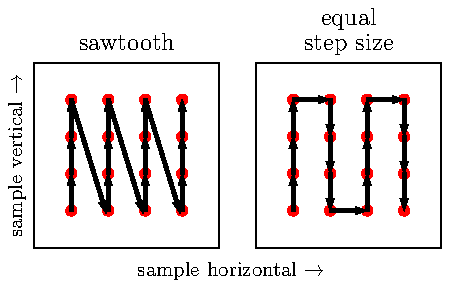
\includegraphics[width=0.75\textwidth]{figures/chap4/rastering_methods.pdf}
	\caption{Schematic of competing raster methods, shown in the sample's reference frame. The clear aperture of the sample is represented by the interior of the black square. The laser propagation direction is out of the page. The laser focal spots are shown as red circles, and the movement of the sample holder relative to the laser focus is indicated by arrows. A 200 $\mu$m border exists between the raster array and the perimeter of the sample's clear aperture. This diagram is to scale for a $1\times1$ mm$^2$ clear aperture sample, a 60 $\mu$m diameter IR focal spot and a 200 $\mu$m step size.}
	\label{fig:Rastering_Methods}
	%figure created using \Python Scripts\rastering\raster_diagram.py
\end{figure}

During the experiment, the sample is rastered across the focus to reduce any deleterious effects of long term uninterrupted laser exposure. During motor movement, the IR beam is blocked with a shutter but the relatively weak XUV beam is allowed to remain on the sample. Each pair of measurements (ground state, excited state) in a delay scan has a unique position on the sample. Typical step sizes are 200 $\mu$m, which is larger than the measured XUV spot size of $\simeq 12 \ \mu \textrm{m}$ and the IR spot size of $\simeq 34 \ \mu \textrm{m}$. Two raster schemes are schematically shown in \cref{fig:Rastering_Methods}. The method shown in the left panel produces a sawtooth pattern on the sample. This method gives very accurate positioning, as the vertical motor is almost always approaching the final position from the same direction. However, the diagonal steps are $\sqrt{N^2 + 1}$ times longer than the vertical steps, where $N$ is the number of vertical steps in the pattern. As a result, there is a bimodal distribution of motor transit times between measurements. If the sample is not fully relaxed between motor movements, this will lead to an inconsistent measurement of the ground state $S_{\textrm{g.s.}}(E)$. Additionally, if the sample is heated by the laser outside of the raster step size, then the average distance between points can affect the measurement of the ground state. The method shown in the right panel alleviates both problems by requiring equal step sizes. Measurements presented in this work were acquired using the method shown in the right panel.

This rastering method has its limitations, as thousands of laser shots hit the sample between each movement. A future upgrade to the beamline could include a rapidly spinning sample mount, as described in \cite{jagerAttosecondTransientAbsorption2018}. Another option would be to directly cool the sample with an \textit{in vacuo} pulsed gas jet pointed at the interaction region, timed such that the valve fires between laser shots.\footnote{Private communication with Prof. Stephen Leone of University of California, Berkeley.}

Before measuring a sample's response for the first time, or after a major optical alignment, an XUV transmission map of the sample must be created. Creating this map serves two purposes: it verifies sample XUV absorption uniformity and it determines the motor coordinates of the sample's clear aperture. To avoid edge effects, the edges of the raster area are chosen to be 200 $\mu$m away from the edge of the clear aperture (see \cref{fig:Rastering_Methods}).

The transient data collection sequence can be summarized as \textit{excited state} $\rightarrow$ \textit{ground state} $\rightarrow$ \textit{move motors}. Details of this sequence are as follows. First, the sample moves to a given raster position and delay wedge position, the IR shutter opens and an excited state spectrum $S_{\textrm{sig}}(\tau, E)$ is recorded. To minimize the duration of the experiment, an XUV reference spectrum $S_{\textrm{vac.}}$ is not recorded. Finally, the sample moves to the next raster position as the delay wedge pair moves to the next delay position. The system is programmed to wait for the wedges to become stationary before the next measurement begins.

Note that in this sequence, the time between the i\textsuperscript{th} excited state and the i\textsuperscript{th} ground state measurement is equal to the exposure time, but the time between the i\textsuperscript{th} ground state measurement and the i+1\textsuperscript{th} excited state measurement is equal to the motor transit time. This sequence is preferable to the alternative (\textit{ground state} $\rightarrow$ \textit{excited state} $\rightarrow$ \textit{move motors}), which would result in a delay step size-dependent relaxation time between the i\textsuperscript{th} excited state and the i+1\textsuperscript{th} ground state measurement.

To further improve our signal-to-noise ratio, we average multiple delay scans together. A typical $\Delta A$ measurement will be repeated between 5 and 50 times. Each delay scan uses the raster points of the previous delay scan so there is a one-to-one mapping of delay to sample position.


\subsection{The Supporting Nitride Membrane}

While most materials have an absorption edge within the range 25 - 150 eV, there are very few commercially available pre-fabricated materials with both the requistite large clear aperture and thickness. Note that either characteristic is relatively easy to achieve individually, but their combination presents unique materials challenges. We considered three synthesis methods to produce this quasi-2D sample:
\begin{enumerate}
	\item sample growth on a traditional substrate, followed by chemical back-etching or milling of the substrate until sub-micron thickness of the heterostructure is achieved;
	\item sample growth on a traditional substrate, followed by mechanical transfer onto a membrane;
	\item sample growth on a membrane.
\end{enumerate}
Sample quality and composition is heavily impacted by local growth conditions such as substrate temperature, deposition rate, substrate crystal cut, substrate-sample lattice mismatch, etc. Many of these characteristics are changed when growing on a substrate of a different cut, or by replacing a substrate with a membrane. In general, one should not expect success when applying a substrate-optimized growth recipe to a freestanding membrane. Therefore, methods 1 and 2 will yield the highest quality samples, as they leverage already-developed sample recipes. However, both methods require a technically difficult second step that is prone to failure.

Selective chemical etching recipes exist for certain compounds, but they usually require an additional chemically intert layer in the heterostructure to protect the sample. Adding this layer will come at the expense of the total XUV flux transmitted by the heterostructure. Additionally, the chemical etching rates are highly dependent on local chemistry, fluid convection and temperature \cite{chiuPhotoluminescenceEvolutionGaAs2015}, which ultimately means that the amount of material removed is uncontrollable and unrepeatable within our requirements (499.9 $\mu$m $\pm$ 10 nm removed from a 500 $\mu$m substrate). For these reasons, we decided to not pursue a chemical etch recipe. Ion or electron milling is more controllable, but too expensive to implement on a large scale. The above reasons preclude the use of Method 1.

Mechanical transfer of thin samples is a tried and true method, but it usually results in flakes with lateral dimensions on the order of 100 $\mu$m. Repeated transfer of many flakes is possible, but there little control over their exact positioning on the membrane. This results in a random distribution of flakes with the possibility of folded or overlapping flakes. These mishaps increase the effective optical density of the sample, changing the IR and XUV absorption properties significantly.

An XUV spatial measurement needs to be taken prior to any ATAS experiment, but a non-uniform distribution of flakes on a membrane would require a much higher resolution map. This is because the flakes are on the order of the XUV and IR focii, so it is critical that the raster points in \cref{fig:Rastering_Methods} correspond to the center of each flake to avoid edge diffraction and to minimize the effects of slow laser pointing drift. For a uniform film, a map can be taken using 200-250 $\mu$m step sizes, as the most important feature is the border of the clear aperture. On the other hand, each flake would have to be sampled $\sim$5 times in each direction to find its center. As a conservative estimate, a membrane covered with $100 \times 100\text{ }\mu$m$^2$ flakes would require a step size of 20 $\mu$m, which increases the number of raster points by a factor of $10^2 = 100$. Considering that a $3 \times 3 \text{ mm}^2$ clear aperture sampled with 200 $\mu$m steps takes $\sim$45 minutes to map, a random distribution of flakes would take a prohibitively long time to map out.

With the first two methods ruled out, we turn to the third method of growing directly on a freestanding membrane. Although it will result in a lower quality sample, it does not have the same technical hurdles of the previous two methods. However, the large clear area makes the heterostructure extremely fragile. We initially attempted to circumvent this problem by using an array of smaller clear apertures.

As shown in \cref{fig:Rastering_Methods}, most of the sample's area isn't directly used by the laser - it exists as a buffer between the grid of sample points. An alternative to a single clear aperture is an array of micro-apertures, each with a diameter on the order of the IR spot size. The micro-apertures exist within a mechanically robust substrate and a thin membrane lies on top of the structure. This configuration significantly eases the material strength requirements by reducing the size of the unsupported area from cm-scale to sub-mm-scale. The regular grid of apertures avoids the difficulties of a randomly distributed sample, easing the XUV mapping step size requirements. Fortunately, these arrays are commercially available from Silson, Norcada (silicon nitride membranes) and US Applied Diamond (diamond membranes) but we encountered technical difficulties in their implementation. Because the aperture size is on the order of the size of the IR focal spot, there is very little room for positioning error, and our motors were insufficiently precise for this application. Further, these arrays are typically only available in at most a $3\times3$ array, which provides an insufficient number of raster points for an ATAS experiment.

\begin{figure}
	\centering
	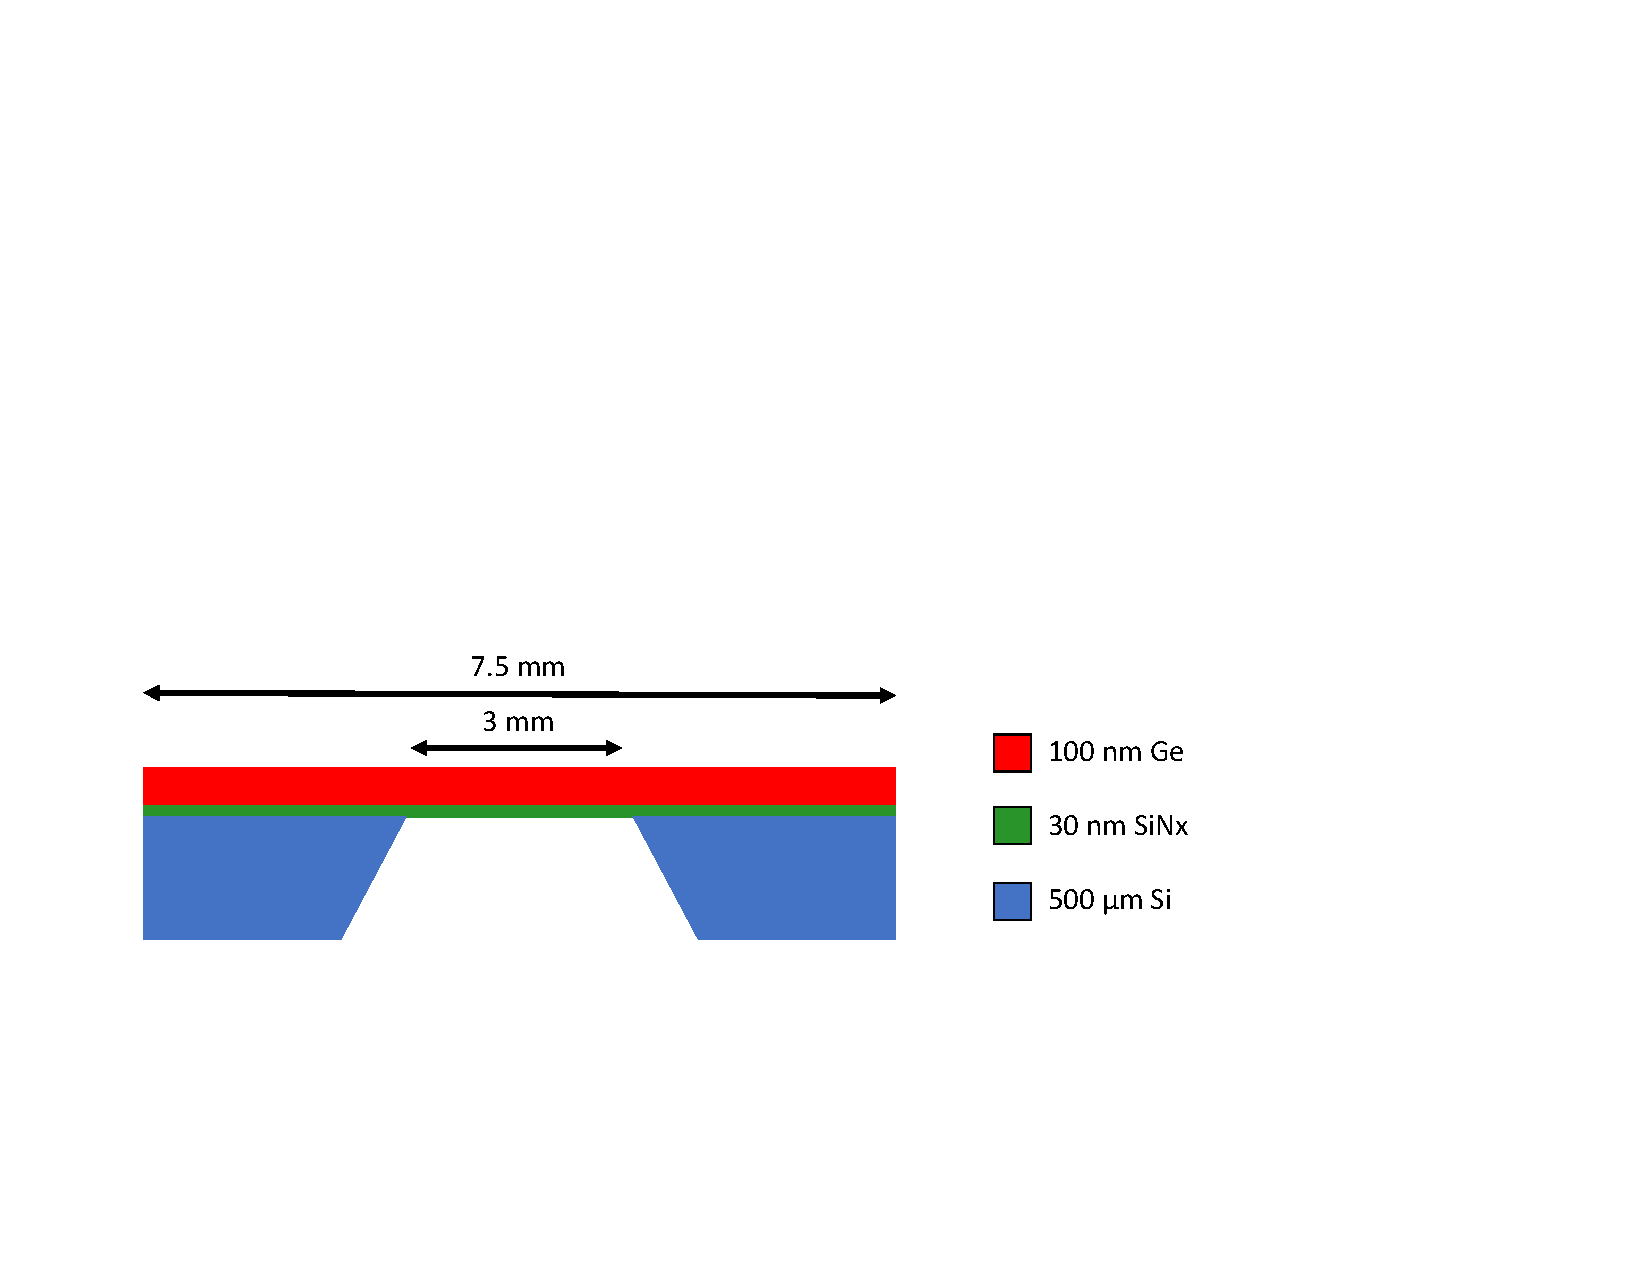
\includegraphics[width=0.75\textwidth]{figures/chap4/Sample_Geometry.pdf}
	\caption{Cartoon showing the cross section of the free standing sample heterostructure. A 500 $\mu$m thick Si frame supports a freestanding 30 nm low stress silicon nitride membrane (Norcada QX7300X), upon which 100 nm of germanium has been deposited. The Si frame has a 3x3 mm$^2$ square clear aperture and a 7.5x7.5 mm$^2$ square external dimension. The taper of the Si frame thickness along the perimeter of the clear aperture forms a knife edge. In an ATAS experiment, the XUV and IR pulses propagate from the top to bottom of the figure.}
	\label{fig:Sample_Geometry}
\end{figure}

With these limitations in mind, we decided to use large aperture x-ray windows from Norcada. These windows consist of a mechanically robust Si frame substrate with a square clear aperture cut through the center. The structure is fabricated so that a thin membrane covers the clear aperture. A schematic of the cross section is shown in \cref{fig:Sample_Geometry}.

\begin{figure}
	\centering
	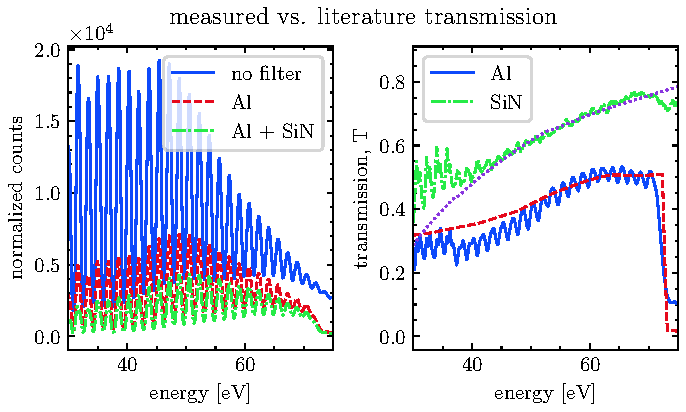
\includegraphics[width=0.75\textwidth]{figures/chap4/SiN_Al_transmission.pdf}
	\caption{XUV transmission measurements of Al metallic filter and silicon nitride membrane. Left panel: normalized XUV counts for i) unfiltered HHG signal, ii) HHG going through a 200 nm Al filter and iii) HHG going through a 200 nm Al filter and 30 nm of silicon nitride. Counts are scaled by the Jacobian. Right panel: transmission curves obtained from the left panel's data. Also shown are literature values for 20 nm of silicon nitride and 200 nm of Al with two 4 nm oxide layers \cite{gulliksonCXROXRayInteractions}. Multilayer interference is not taken into account. Oscillations in measured transmission are numerical artifacts originating from a finite detector noise floor and XUV brightness instabilities.}
	\label{fig:SiN_Al_transmission}
	% dataset: \2019_05_02\
	% plotted using: \Python Scripts\Spectrometer\test\nitride_trans.py
\end{figure}

Norcada offers these structures with either a silicon (polycrystalline or single-crystal) or a silicon nitride membrane. An ideal membrane is transparent to both XUV and IR wavelengths with a high damage threshold. Referring to \cref{fig:Sample_trans_CXRO}, 100 nm of Si provides a relatively flat transmission curve from 25 to 100 eV. In constrast, 30 nm of silicon nitride has poor, but featureless, transmission at lower energies. Both materials transmit light below their bandgaps (5 eV for SiN and 1.14 eV for Si). Finally, silicon nitride's higher bandgap results in a significantly higher laser damage threshold \cite{gamalyAblationSolidsFemtosecond2002,austinFemtosecondLaserDamage2018,keldyshIonizationFieldStrong1965}. Taking all these factors into account, we decided to use 30 nm silicon nitride membranes for germanium transient absorption experiments. The measured transmission of a typical membrane is shown in \cref{fig:SiN_Al_transmission}.

\begin{figure}
	\centering
	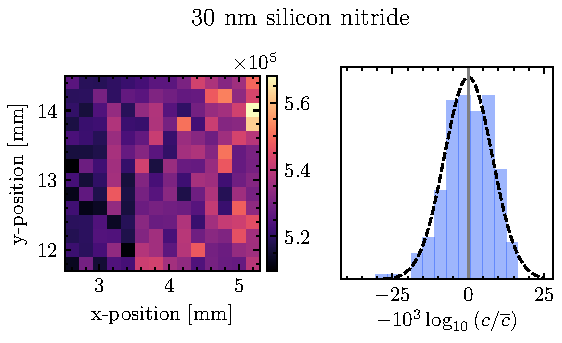
\includegraphics[width=0.75\textwidth]{figures/chap4/nitride_map.pdf}
	\caption{XUV transmission map of 30 nm silicone nitride freestanding membrane. Left panel: integrated XUV counts in the range 30 -- 34 eV. Sample holder motor positions are indicated by x- and y-positions. Right panel: histrogram of logarithmic deviation of counts from the average. Dashed line shows a normal distribution.}
	\label{fig:nitride_map}
	% figure created using \Python Scripts\Spectrometer\test\rastermap.py
	% dataset: C:\testdata\2019_09_10\4_55_32 PM_nitride_map1
\end{figure}

The commercial membranes have very uniform transmission, as shown in \cref{fig:nitride_map}.

\subsection{Laser Damage}
\label{sec:laser_damage}

\begin{figure}
	\centering
	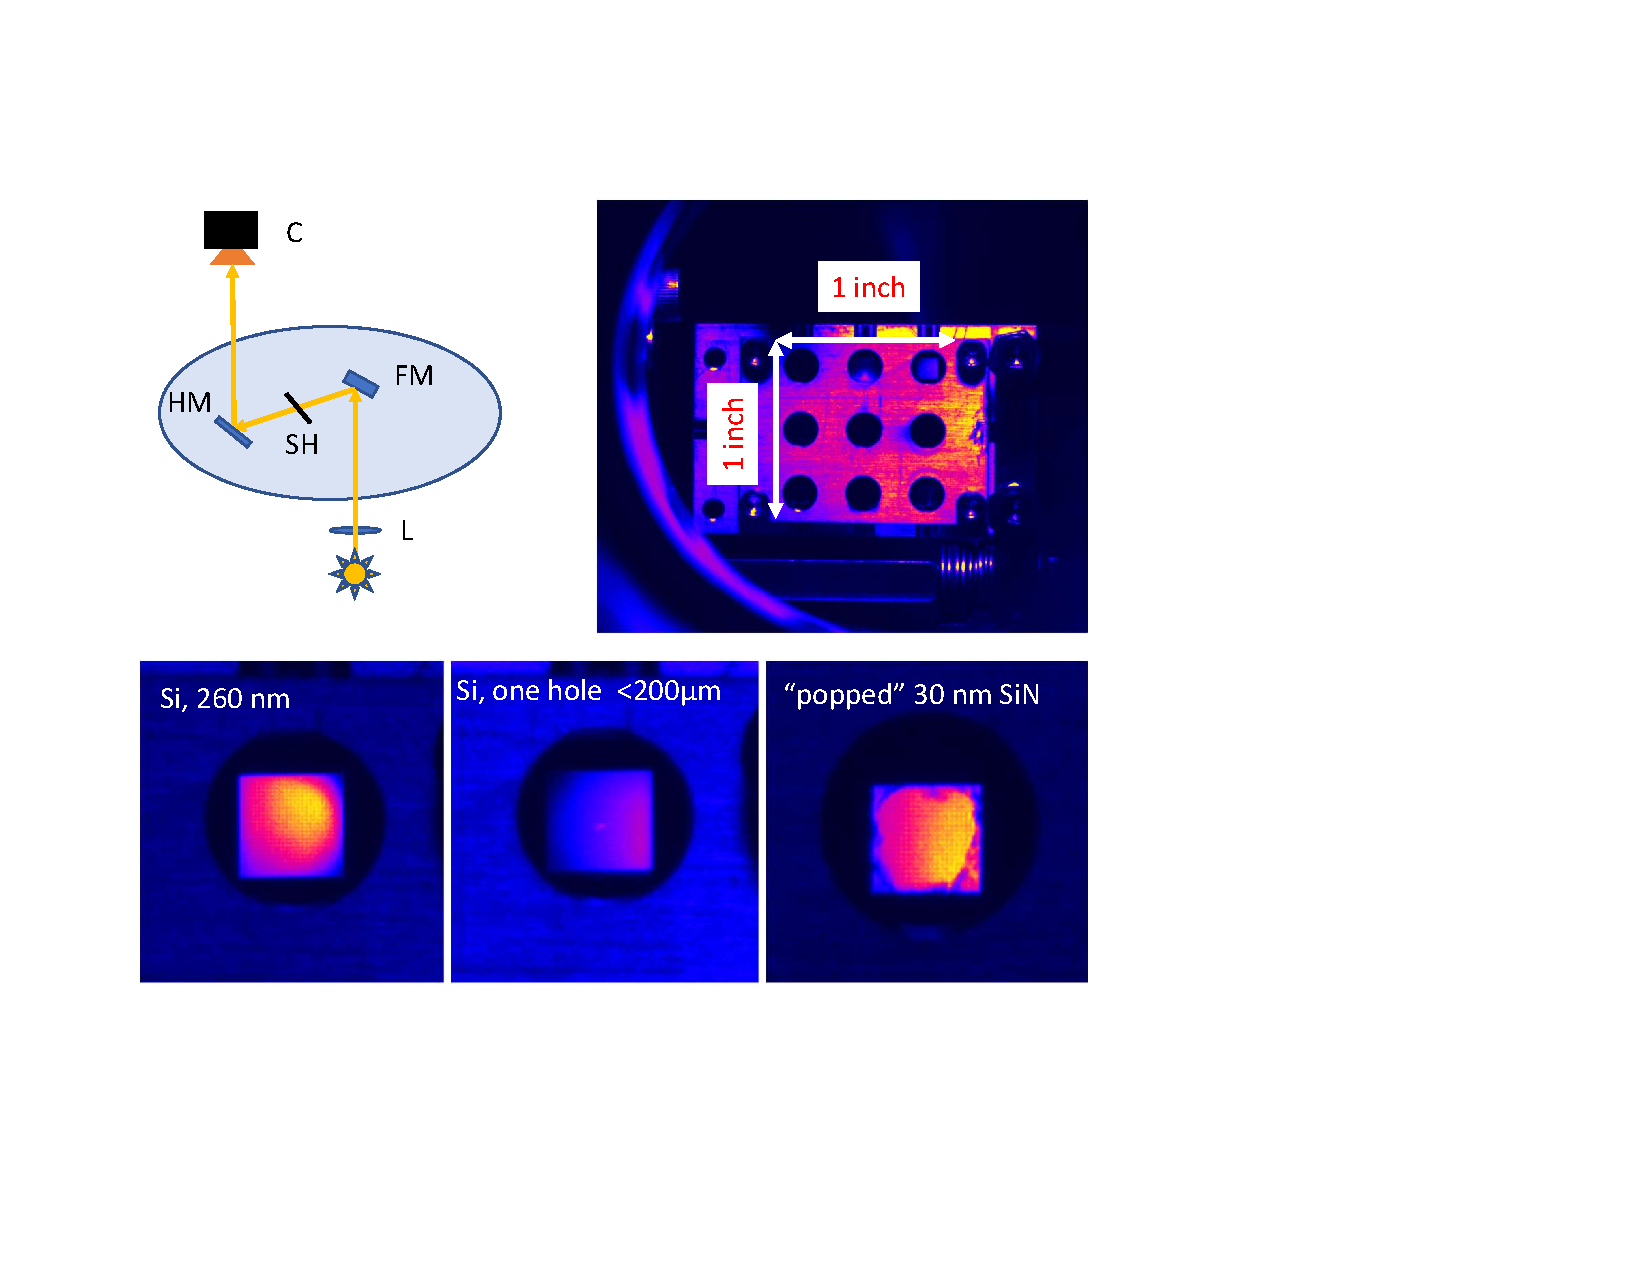
\includegraphics[width=0.75\textwidth]{figures/chap4/sample_holder_damage.pdf}
	\caption{\textit{In-situ} imaging of the samples within the target chamber. Left: optical setup for \textit{in-situ} imaging of samples. C: Si CCD camera, HM: hole mirror, SH: sample holder, FM: translatable silver mirror, L: lens. Right: false color image showing the sample holder with a 3 x 3 grid of 5 mm diameter clear apertures. Samples are held in a clamshell design centered in the clear apertures and are backlit using a flashlight.}
	\label{fig:sample_holder_damage}
\end{figure}

\begin{figure}
	\centering
	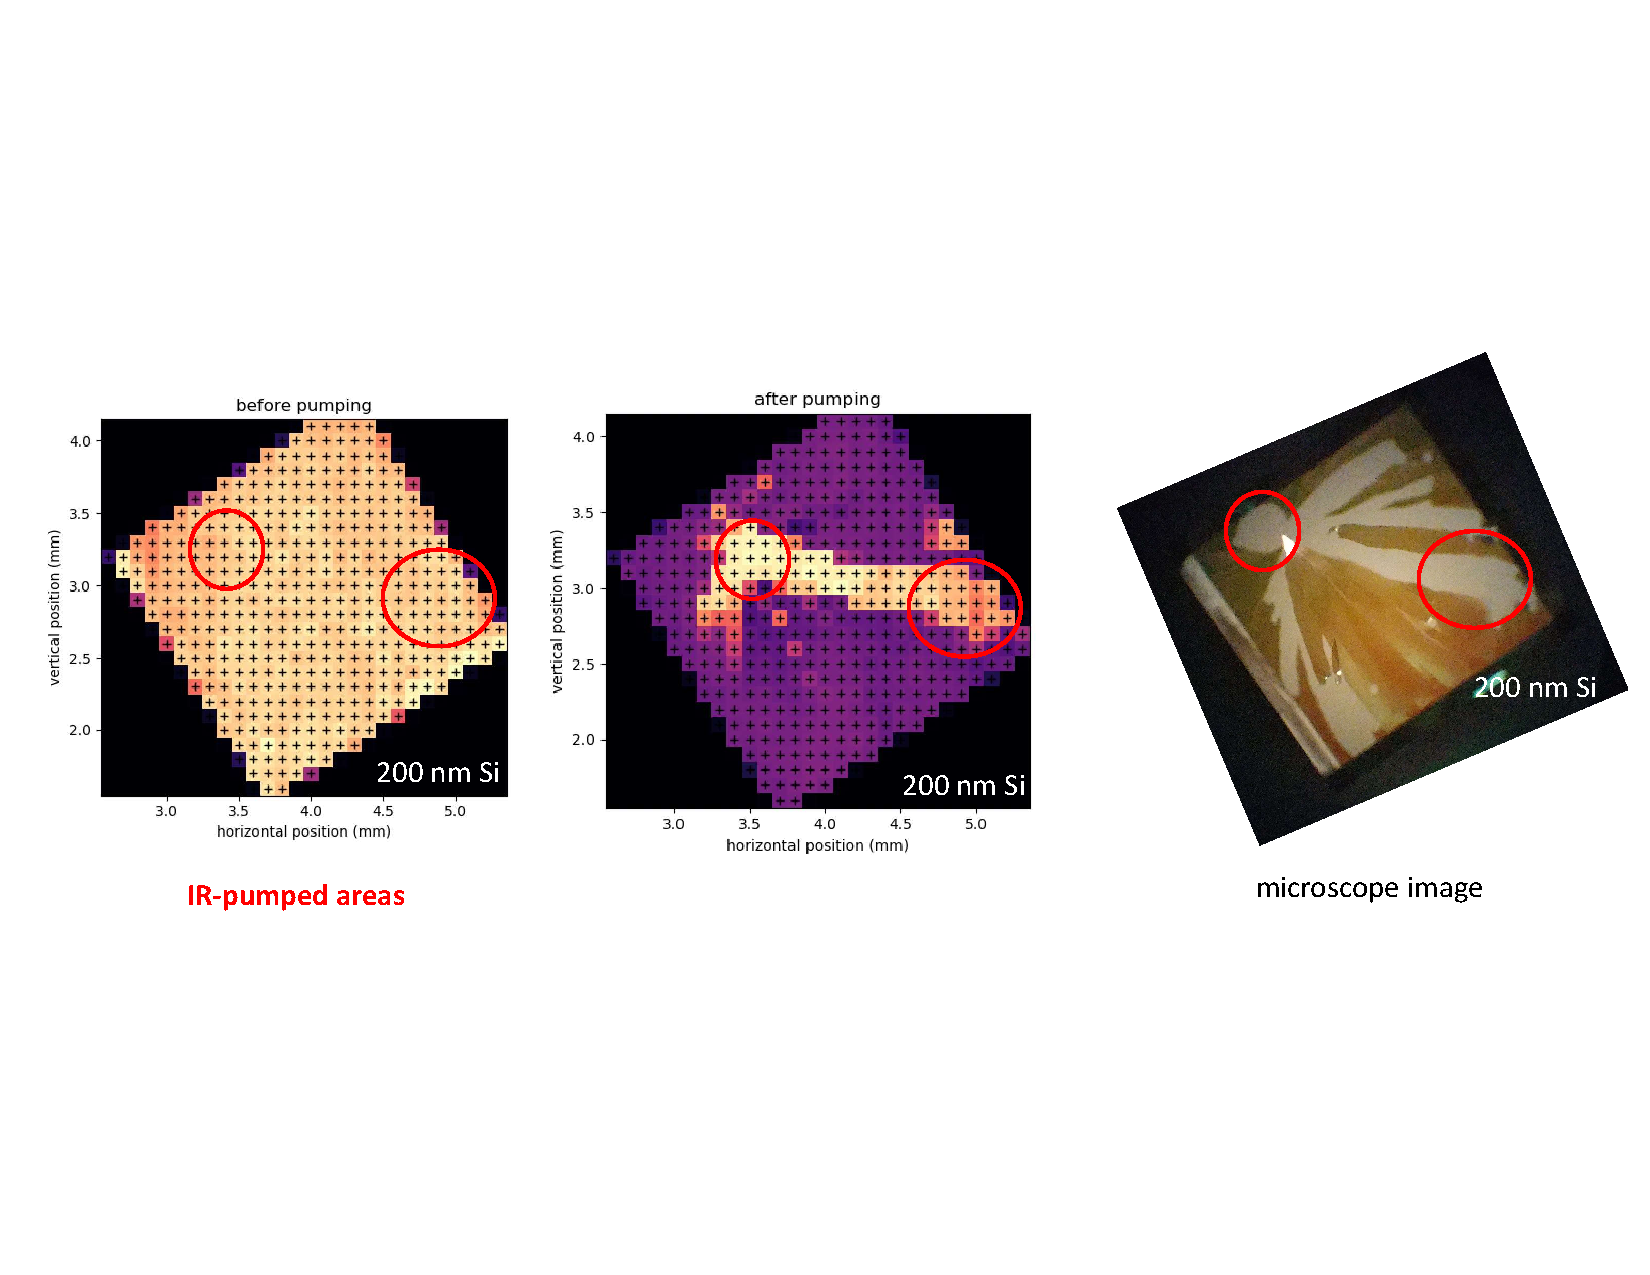
\includegraphics[width=0.9\textwidth]{figures/chap4/Si_damage.pdf}
	\caption{Laser damaged 200 nm silicon membrane samples. Left panel: XUV map of pristine Si before being exposed to IR laser. Center panel: XUV map of damaged sample after being pumped with $\approx \text{ 65 }\mu$J of $\lambda = 1500 \text{ nm}$ at 1 kHz rep. rate in two locations. Right panel: microscope image of damaged sample (beige) showing large sections of missing material (white). Red circles in all three pictures indicate the two locations that were exposed to IR laser light.}
	\label{fig:Si_damage}
\end{figure}

Unlike the gas samples traditionally used in the DiMauro lab, condensed matter samples can suffer permanently laser-induced damage which frustrates any intensity-dependent investigation. The delicate nature of a $\simeq 100 \ \textrm{nm}$ freestanding membrane further complicates these studies. The exact damage mechanism was not studied but we have observed two modes of membrane failure, which will be discussed presently. Occasionally, the volume near the IR focal spot will be ablated by the laser, leaving the rest of the freestanding sample undamaged. The most common failure mode results in the immediate destruction of the entire membrane, often within a single camera exposure ($\simeq 1$ second).

Sample damage is apparent in both the visible and the XUV. The top left panel of \cref{fig:sample_holder_damage} shows our \textit{in-situ} method of imaging the samples using visible light. The top right panel shows a false color image of our sample holder within the chamber. The $3 \times 3$ grid of 5 mm diamter clear apertures is visible as dark circles. The bottom three panels of \cref{fig:sample_holder_damage} show close ups of three samples. On the left, we have a pristine Si membrane; in the middle panel, we have a Si membrane with a $< 200 \ \mu \textrm{m}$ laser-drilled pinhole (visible as a bright point in the center of the membrane); the right panel shows a completely obliterated SiN membrane (visible as ragged edges).

\cref{fig:Si_damage} shows a 200 nm thick freestanding Si membrane before and after it was laser damaged. The first two panels show the integrated XUV transmission ($E \simeq 60-100 \ \textrm{eV}$) as the sample is rastered across the XUV focus; each image consists of over 100 individual measurements. The small black ``+'' signs correspond to the center of the coordinates for each exposure, and the sample is rotated $\simeq 30$ degrees relative to the motor axes. In the left panel, we see the XUV transmission  of a pristine sample before it was exposed to the IR laser. The center panel shows the same sample shortly after it was briefly pumped with $\simeq 65 \ \mu \textrm{J}$ of $\lambda=1500 \ \textrm{nm}$ light at 1 kHz in the two locations indicated by red circles. Damage occured within the first camera exposure (2 seconds). We see high transmission (beige) in a horizontal stripe across the membrane; the remaining parts of the sample have lower transmission (purple), although there are signs of increased transmission in the bottom-center area of the sample. The right panel shows a microscope image of the sample after it was removed from the chamber. We can see that while the areas exposed to the laser are missing, the entire membrane is shattered and is unusable.

Ultrafast melting has been identified as a possible mechanism for mid-IR laser induced damage \cite{austinSemiconductorSurfaceModification2017,austinFemtosecondLaserDamage2018}, which can be understood as the following. At the microscopic level, the germanium lattice consists of a multitude of electronic bonds between valence electrons. In the ground state, there exists an energetic balance between the attractive bonding force and an electrostatic repulsion of inner electrons \& nuclei. As the VB electrons are excited to the CB, the attractive force is weakened and the bond distance increases. If we continue to excite the VB, it will become depleted to the point where the repulsive forces destroy the bonds. Thereafter, the material no longer resists shear forces - much like a liquid. Experiments have shown that the lattice is destroyed within 100 fs after the electron-hole plasma is created, and the crystal melts 500 fs later. In semiconductors, tight-binding calculations predict that ultrafast melting occurs when the conduction band density $N_{\textrm{CB}}$ is about 8-12\% of the valence band density $N_{\textrm{VB}}$ \cite{stampfliTheoryLaserinducedInstability1990,austinFemtosecondLaserDamage2018}.

We estimate the valence band electron density of the ground state as the product of the number of valence electrons per atom and the number of atoms per unit cell divided by the unit cell volume. Germanium has a diamond cubic lattice with a unit cell volume of ${a^3 = (5.658 \ \AA)^3 = 1.81129 \times 10^{-22} \ \textrm{cm}^3}$, and an electron configuration of ${[\textrm{Ar}] 3\textrm{d}^{10 }4\textrm{s}^2 4\textrm{p}^2}$. With 8 atoms per unit cell and 4 valence electrons per atom, the valence band electron density of the ground state is $N_{\textrm{VB}} = 1.767 \times 10^{23} \ \textrm{cm}^{-3}$. Therefore, we would not expect ultrafast melting to occur unless $N_{\textrm{CB}}$ exceeds $\simeq 1.767 \times 10^{22} \ \textrm{cm}^{-3}$.

\textbf{slower heating (average power)}

two mechanisms of sample damage (microscopic level): slower heating (average power) vs instaneous damage (peak power)

two ways samples get destroyed (macroscopic level): pinhole drilled vs membrane popped.

%\subsection{Estimation of Excited Carrier Density}
%\label{sec:estimate_excited_carrier_density}
%
%We are concerned with two quantities: the peak excitation fraction in the sample and the average excitation fraction at the location of the XUV focus. The former quantity is relevant when considering sample damage, whereas the latter will be proportional to the measured signal. If the XUV and IR spots are perfectly overlapped at the sample plane, then these two quantities are approximately equal. We first calculate the peak excitation fraction, then we consider how a misaligned beam will affect the measured signal.
%
%The laser propagation calculations in \cref{fig:pump_on_focus_calculation} were done for vacuum, but we are concerned with the field in our sample. The electric field inside a dielectric $E_{\text{int}}$ is related to the external electric field by the following equation \cite{schultzeAttosecondBandgapDynamics2014}:
%\begin{equation}
%E_{\text{int}} = \frac{2}{1+\sqrt{\epsilon}} E_{\text{ext}}
%\label{eqn:internal_external_Efield}
%\end{equation}
%where $E_{\text{int}}$ is the electric field inside the sample, $E_{\text{ext}}$ is the electric field outside the sample, $\epsilon$ is the dielectric constant and its square root is the refractive index $n_{\text{IR}}$. The internal intensity $I_{\text{int}}$ is the square of the internal electric field. For germanium at $\lambda$ = 1430 nm, $n_{\text{IR}}$ = 4.2481, and we have the following relations:
%\begin{equation}
%\begin{aligned}
%E_{\text{int}} &= 0.381 \times E_{\text{ext}} \\
%I_{\text{int}} &= 0.145 \times I_{\text{ext}}
%\end{aligned}
%\end{equation}
%
%Given our laser paremeters, we can estimate the highest carrier density within the sample. First, we estimate the absorbed laser fluence, $F_{\text{abs}}$ \cite{harbCarrierRelaxationLattice2006}:
%\begin{equation}
%F_{\text{abs}} = F_{\text{inc}} \left(1-R\right) \left( 1-\exp(-\alpha L) \right) \left(1+R \exp(-\alpha L)\right),
%\label{eqn:absorbed_fluence}
%\end{equation}
%where $F_{\text{inc}}$ is the incident fluence, $R$ is the reflectivity equal to the square of the Fresnel coefficient, $\alpha$ is the absorption coefficient and $L$ is the sample thickness. The bracketed terms in \cref{eqn:absorbed_fluence} are the fraction of fluence transmitted by the first surface, the fraction absorbed by a single pass through the sample, and the additional absorption due to a back reflection off the rear face of the sample. Note that the back-propagating beam will arrive (on average) at a delay of $n_{\text{IR}} L/(2c) \approx 0.7 \text{ fs}$ later than the forward-propagating beam. This time scale is nearly two order of magnitude less than the IR pulse duration, so we should expect any electron dynamics initiated by the back reflection to contribute to the measured signal.
%
%If each absorbed photon corresponds to an excited electron, then the excited carrier density $\Delta N$ is given by the following expression \cite{cushingDifferentiatingPhotoexcitedCarrier2019}:
%\begin{equation}
%\Delta N = \frac{F_{\text{abs}}}{\hbar \omega} \frac{1}{L},
%\label{eqn:excitation_fraction}
%\end{equation}
%where $\hbar \omega$ is the IR photon energy. In \cref{eqn:excitation_fraction}, the quantity $F_{\text{abs}} / (\hbar \omega)$ represents the number of absorbed photons per unit area; dividing this quantity by the sample thickness gives the number of absorbed photons per unit volume. This assumes that the skin depth of the material is greater than membrane thickness, which is true for germanium at these wavelengths.
%
%Finally, we convert the excited carrier density to a fractional excitation. Germanium has $N_{\text{u.c.}}=2$ valence electrons per unit cell, and each unit cell has a volume $V_{\text{u.c.}}=4.527 \times 10^{-23} \text{ cm}^{3}$. Therefore the fractional carrier excitation is
%\begin{equation}
%f = \Delta N \frac{V_{\text{u.c.}}}{N_{\text{u.c.}}}
%\end{equation}
%
%We can use literature values for 100 nm of germanium pumped at $\lambda$ = 1430 nm light. From the literature \cite{nunleyOpticalConstantsGermanium2016}, $R = 0.38315$, $\alpha = 5803.4 \text{ cm}^{-1}$, and so $F_{\text{abs}} = 0.0413 \times F_{\text{inc}}$. Therefore, only about 4.13\% of the incident fluence is absorbed by the sample.
%
%According to the calculations in \cref{fig:pump_on_focus_calculation}, for each 1 $\mu$J energy input pulse (measured at L4), 0.413 $\mu$J makes it to the focal plane. 49\% of that energy is within the main lobe, which contains 0.202 $\mu$J of energy. Approximating the central lobe as a Gaussian beam with a FWHM of 35 $\mu$m and a pulse energy of 0.202 $\mu$J, the peak fluence is calculated by dividing the total energy of the Gaussian by $\pi w^2/2$. The Gaussian beam waist $w$ is related to the FWHM via $w^2 = \text{FWHM}^2 / (2 \ln 2)$. Thus, for each 1 $\mu$J input energy, the peak fluence in the central lobe is 14.6 mJ/cm$^2$ and the absorbed peak fluence is 0.60 mJ/cm$^2$. This corresponds to an peak excited carrier density of $4.3 \times 10^{20} \text{ cm}^{-3}$ and an excitation fraction of 0.98\% (per 1 $\mu$J of input energy).

\section{Finite Beam Size Considerations: Measuring $\Delta A$}
In a transient absorption experiment, we measure the change in absorbance of the sample in response to a laser-induced electronic excitation. We measure macroscopic properties in the lab, but the coefficients are determined by the local conditions at the microscopic level. In this section, we will describe how the two quantities are related given the XUV and excited fraction spatial profiles. We will use this formalism to calculate the sensitivity of our measurement to the relative spot sizes of the IR excitation laser and the XUV probe beam. Additionally, we will calculate the sensitivity of the measurement to misalignment of the two focal spots.

\subsection{Relating Macroscopic and Microscopic Absorbance}
\label{sec:micro_macro_DeltaA}

The XUV absorption within the sample is linear, so we can write the measured spectrum $S_i$ as the product of the input XUV brightness $I_{\textrm{XUV}}$ and a transmission factor $T_i$:
\begin{equation}
\begin{aligned}
S_i(E, \tau) &= I_{\textrm{XUV}}(E) \ T_i(E, \tau), \\
\textrm{with} \ T_i &= 10^{- A_i}, \\
\textrm{and} \ A_i &= \int_{0}^{L} \alpha_{10}(E, z) \dd{z},
\end{aligned}
\label{eqn:DeltaA_macro}
\end{equation}
where $A_i$ is the absorbance and $S_i(E,\tau)$ is the recorded XUV spectrum with photon energy $E$ at XUV-IR delay $\tau$. The subscript $i$ denotes a ground state (g.s.) or excited state (e.s.) measurement. Note that \cref{eqn:DeltaA_macro} assumes no transverse spatial structure of the ionization fraction or the XUV light, so $S_i, \ I_{\textrm{XIV}}, \ T_i, \ A_i$ and $\alpha_{10}(z)$ are effectively macroscopic quantities. In our experiments, we measure the area integral of the spectrum in the far-field:
\begin{equation}
S_{\textrm{meas},i} = \iint \dd{x} \dd{y} I_{\textrm{XUV}}(x,y) \ t_i(x,y),
\end{equation}
where $t_i(x,y)$ is the \textit{local transmission} of the sample/heterostructure at sample position $(x,y)$.\footnote{In the following discussion, we drop the explicit energy- and time-dependence to make the equations more readable. The time dependence comes from the evolution of the ionization fraction $\eta$, and the energy dependence comes from the energy-dependent excitation and ground state of the sample. Also note that the XUV beam shape does not appreciably change over the sample thickness (since $z_R \simeq 1 \ \textrm{mm} \gg 100 \ \textrm{nm}$), so we omit the $z$-dependence in writing $I_{\textrm{XUV}}(x,y)$.}  Therefore, the (macroscopic) transmission and absorbance of the excited or ground state relative to a vacuum reference can be expressed as:
\begin{equation}
\begin{aligned}
T_i &= \frac{S_i}{S_{\textrm{vac.}}} = \frac{\iint \dd{x} \dd{y} I_{\textrm{XUV}}(x,y) \ t_i(x,y)}{ \iint \dd{x} \dd{y} I_{\textrm{XUV}}(x,y)} \\
A_i &= - \log_{10}(T_i)
\end{aligned}
\end{equation}
Using this notation, the \textit{change in absorbance} between the excited and ground states is:
\begin{equation}
\Delta A \equiv A_{\textrm{e.s.}} - A_{\textrm{g.s.}} = - \log_{10} \left( \frac{\iint \dd{x} \dd{y} I_{\textrm{XUV}}(x,y) \ t_{\textrm{e.s.}}(x,y)}{\iint \dd{x} \dd{y} I_{\textrm{XUV}}(x,y) \ t_{\textrm{g.s.}}(x,y)} \right)
\label{eqn:Delta_A_2}
\end{equation}
Now, let us write the cross section $\alpha$ of the sample as a ground state term plus an ionization-dependant perturbation term:
\begin{equation}
\begin{aligned}
\alpha(x,y,z) &= \alpha_{10} (1 + \eta(x,y,z)) \\
\textrm{with} \quad \alpha_{10} &\equiv \frac{\alpha_e}{\ln 10} = \frac{4 \pi \Im [\tilde{n}]}{\lambda \ln 10}.
\end{aligned}
\end{equation}
From \cref{eqn:DeltaA_macro}, the absorbance of a sample of thickness $L$ is:
\begin{equation}
\begin{aligned}
A_{\textrm{g.s.}} &= \alpha_{10} L, \\
A_{\textrm{e.s.}} &= (\alpha_{10} + \bar{\eta}_z(x,y)) L.
\end{aligned}
\end{equation}
where we have defined the \textit{depth-averaged excitation fraction}, $\bar{\eta}_z(x,y)$ as:
\begin{equation}
\bar{\eta}_z(x,y) \equiv \frac{1}{L} \int_{0}^{L} \eta(x,y,z) \dd{z}.
\label{eqn:eta_z}
\end{equation}
Since $t_{\textrm{g.s.}}(x,y)$ is spatially invariant, \cref{eqn:Delta_A_2} simplifies to:
\begin{equation}
\Delta A = -\log_{10} \left( \frac{ \iint \dd{x} \dd{y} I_{\textrm{XUV}}(x,y) 10^{- \alpha_{10} L \bar{\eta}_z(x,y)}}{ \iint \dd{x} \dd{y} I_{\textrm{XUV}}(x,y)} \right).
\label{eqn:Delta_A_3}
\end{equation}
Therefore, the measured macroscopic sample response is the integral of the local absorbance weighted by the local XUV probe intensity. \cref{eqn:Delta_A_3} will reduce to the \cref{eqn:DeltaA_macro} if and only if $\bar{\eta}_z(x,y)$ is constant for all values of $x$ and $y$. Since $\bar{\eta}_z(x,y)$ is created in response to the IR laser, this is equivalent to making the plane wave approximation for the pump arm. In the case of finite excitation and probe beams, the measured macroscopic response of the sample will always be lower than that predicted by the \textit{peak excitation fraction}, $\textrm{Max}[\eta(x,y,z)]$. 

Our condensed matter experiments are limited by our ability to measure weak signals. We can improve the measured signal by increasing the depth-averaged excitation fraction, but we are constrained by the ultrafast melting condition ($N_{\textrm{CB}} \simeq 0.1 N_{\textrm{VB}}$), which puts an upper limit on the peak excitation fraction $\textrm{Max}[\eta(x,y,z)]$. Our detection efficiency, defined as the measured $\Delta A$ divided by $\Delta A$ at the peak excitation fraction, is an important experiment parameter. In the following disussion, we consider the effect of the transverse profile on the measurement efficiency. In \cref{sec:thin_film_interference} we will see that the thin film interference causes a strong $z$-dependence of $\eta(x,y,z)$ that will further diminish the measurement efficiency.

We can gain intuition about the situation by numerically evaluating \cref{eqn:Delta_A_3} using mathematically convenient expressions for $I_{\textrm{XUV}}$ and $\bar{\eta}_z$:
\begin{equation}
\begin{aligned}
I_{\textrm{XUV}} (x,y,z) &= \frac{2}{\pi w(z)^2} \exp \left( - \frac{2 (x^2 + y^2)}{w(z)^2} \right), \\
\bar{\eta}_z(x,y) &= \eta_0 \exp \left( -\frac{2(x^2 + y^2)}{w_1^2} \right), \\
\textrm{with} \ w(z) &= w_0 \sqrt{1 + (z/z_R)^2}, \\
\textrm{and} \ w_1 &\equiv a*w_0.
\end{aligned}
\label{eqn:XUV_eta_expressions}
\end{equation}
In the above, we have made the radius of the depth-averaged excited fraction $a$ times larger than the XUV spot radius. Additionally, the XUV intensity is normalized such that the denominator in \cref{eqn:Delta_A_3} evaluates to $1$. In \cref{fig:Delta_A_curve}, we numerically integrate \cref{eqn:Delta_A_3} using the assumptions of \cref{eqn:XUV_eta_expressions} to better understand the importance of the relative sizes the XUV and depth-averaged ionization fraction spot sizes. The left panel shows the efficiency of measuring the amplitude $\eta_0$ for a given ratio of spot sizes. We see an error function-like curve which approaches unity as $a \rightarrow \infty$, which is consistent with the plane wave approximation. Equal spot sizes result in a measured $\Delta A$ that is only 40.7\% of the amplitude $\alpha_{10} L \eta_0$, and an XUV spot size 1/3 of the excited fraction results in an efficiency of 89\%. In our experiment, the XUV beam waist radius is $\simeq 6 \ \mu \textrm{m}$ and the IR FWHM is $\simeq 34 \ \mu \textrm{m}$, which yields $a \simeq 5$ and a detection efficiency of $\simeq 96\%$. In the right panel, we plot the expected measured signal as a function of the effective excitation cross section for different values of $a$.

Note that we obtain $a=5$ using our XUV optic with a demagnification factor of 3. If instead we used a 1-to-1 toroid to focus the XUV onto the sample, we would have $a=5/3$, and the measurement efficiency would be $\simeq 65\%$. Therefore, the ellipsoid's demagnification yields a 50\% increase in signal compared to a 1-to-1 toroid.

\begin{figure}
	\centering
	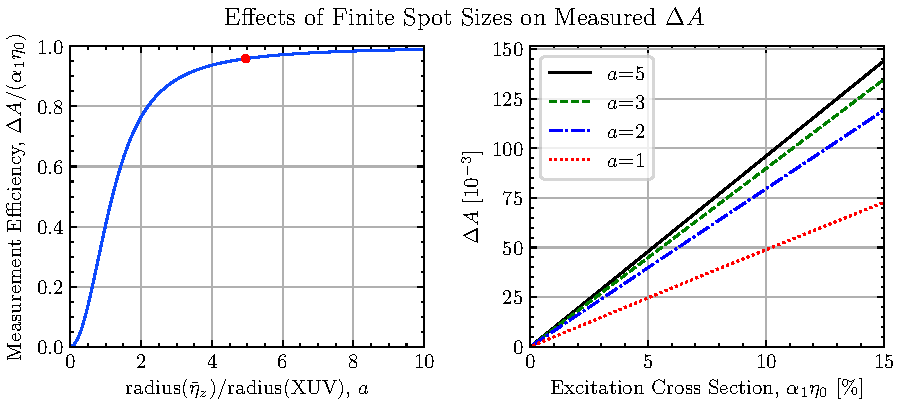
\includegraphics[width=0.9\textwidth]{figures/chap4/Delta_A_curves.pdf}
	\caption{The effect of finite pump and probe sizes in measuring the change in absorbance in an ATAS experiment. Left panel shows the relative sensitivity of $\Delta A$ as a function of the relative sizes of the XUV and $\bar{\eta}_z$ spots. The red dot represents our experimental configuration ($a\simeq 5$), which yields $\simeq 96\%$ measuring efficiency. The right panel shows the expected $\Delta A$ amplitudes as a function of both $a$ and $\alpha_{10} L \eta_0$. See \cref{eqn:Delta_A_3} and surrounding text for details.}
	\label{fig:Delta_A_curve}
	% plot made with \Python Scripts\DrakeIonization\plot_DeltaA_function.py
\end{figure}


\subsection{XUV-IR Misalignment}

\begin{figure}
	\centering
	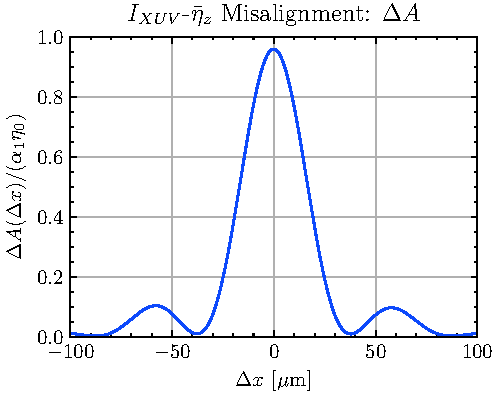
\includegraphics[width=0.75\textwidth]{figures/chap4/XUV_eta_misalignment.pdf}
	\caption{The effect of relative misalignment of the IR and XUV spots. We assume linear excitation of the sample for this calculation.}
	\label{fig:XUV_eta_misalignment}
	% plot made with \Python Scripts\DrakeIonization\VolumeAveraging_class_script.py
\end{figure}

We now consider the effect of having slightly misaligned IR and XUV spots. For this calculation, we assume the sample excitation is purely linear: $\eta(x,y) \propto I_{\textrm{IR}}(x,y)$. We numerically integrate \cref{eqn:Delta_A_2} using the simulated IR intensity profile $I_{\textrm{IR}}(x,y)$ from \cref{fig:pump_on_focus_calculation} and an XUV spot with a 6 $\mu$m waist and a transverse offset of $x \rightarrow x+\Delta x$. The result is shown in \cref{fig:XUV_eta_misalignment}. As in \cref{fig:Delta_A_curve}, we see that the finite beam sizes lead to a maximum measurement effiency of about 96\%. The measurement is very sensitive to misalignment; a 10 $\mu$m offset will reduce the efficiency to 76\%, a 20 $\mu$m deviation yields 37\%, and the minimum of $\simeq 0.8\%$ is near $\Delta x = \pm 37 \ \mu \textrm{m}$. The local maximum at $\Delta x = \pm 58 \ \mu \textrm{m}$ is due to the \nth{1} lobe of the IR diffraction pattern, yielding an efficiency of $\simeq 10\%$.

%We have yet to calculate the sensitivity of spatial overlap to deviations in the input laser pointing.
In our chamber, a 10 $\mu$m displacement of the IR at the sample corresponds to a 15 $\mu$rad tilting of the hole mirror (HM). There are two ways misalignment can affect experimental results. If the relative positions of the XUV and IR focal spots changes as an experiment is performed, then the recorded ATAS signal would be a function of both the laser-induced dynamics and the XUV-IR spatial misalignment. On the other hand, if the entire experiment is performed using a constant misalignment, we would be exciting the sample to some peak excitation fraction $f$, but our probe would be measuring a lower excitation fraction ($\approx f a / a_{max}$). Consequently, the measured ATAS signal would be lower than otherwise expected, and any attempts to boost the signal by increasing the interaction intensity could result in permanent laser-induced sample damage.

A condensed matter ATAS experiment has much tighter alignment tolerances than a gas phase experiment. This discrepancy is a simple consequence of sample geometry and density. In either experiment, the measured signal comes from the region of space where the sample density, XUV intensity and IR intensity overlap. The transmission of XUV through the sample is, to first order, $T= \exp(- n \mu_a L)$, where $n$ is the number density, $L$ is the sample thickness and $\mu_a$ is the photoabsorption cross section. As discussed above, for technical reasons the experiment should be designed with $T \approx 1/2$. Therefore, the product $n \mu_a L$ will be approximately constant for any transient absorption experiment.

The number density of a condensed phase sample is determined by the chemistry of the compound and is on the order of $4 \times 10^{22} \text{ atoms}/\text{cm}^3$. The experimentalist is free to engineer clever sample geometries, heterostructures and/or nanopatterns, but the high atomic density (and thus absorption coefficient) dictates a total sample thickness on the order of 100 nm. On the other hand, the spatial profile and density of a gas phase sample is determined by the gas nozzle design and its backing pressure, respectively. A typical nozzle used in our lab produces a gas plume with lateral dimensions on the order of 200 - 500 $\mu$m. This effectively creates a sample that is three orders of magnitude thicker than a condensed phase sample, which relaxes the alignment constraints significantly. This has important consequences for the alignment of the sample.

If the XUV and IR are perfectly collinear, then the beam overlap region is effectively infinite in the propagation direction. In this case, the measured $\Delta A$ will be finite regardless of any displacement of the sample plane from the focal plane, and maximal when the sample lies in the focal plane. However, if there is a small angle $\delta \theta$ between their $k$-vectors, then the beams will only spatially overlap within a finite region. In this case, the position of the sample plane relative to the beam crossing plane becomes a critical experimental parameter. For an infinitely thick sample (i.e., a chamber effusively filled with gas), it wouldn't matter where the beams crossed as long as they overlapped somewhere within the chamber. Then, the XUV-$\eta$ overlap integral would decrease as a function of $\delta \theta$, but it would never go to zero. For a thin sample, the bounds of \cref{eqn:eta_z} must enclose the beam overlap region, or else the integral will be zero. Thus, the signal strength of a condensed phase ATAS experiment is roughly 3 orders of magnitude more sensitive to the $z$-position of the sample relative to the focal plane than a gas phase ATAS experiment.


\section{Nonlinear Excitation of Germanium}
\label{sec:nonlinear_excitation_germanium}

\begin{table}[]
	\centering
	\begin{tabular}{ll}
		{\ul effective electron masses} &  \\
		$m_{\textrm{CB}}$, for direct transitions & $0.041 * m_e$ \\
		$m_{\textrm{CB}}$, for indirect transitions & $0.0815 * m_e$ \\
		$m_{\textrm{VB}}$, from HH & $0.33 * m_e$ \\
		$m_{\textrm{VB}}$, from LH & $0.043 * m_e$ \\
		$m_{\textrm{VB}}$, from SO & $0.084 * m_e$ \\
		&  \\
		{\ul ground state band gaps} &  \\
		direct transitions, from LH/HH & 0.8 eV \\
		direct transitions,  from SO & 0.828 eV \\
		indirect transitions,  from LH/HH & 0.67 eV \\
		indirect transitions, from SO & 0.668 eV \\
		&  \\
		electron-phonon collision time, $\Gamma^{-1}$ & 47 fs
	\end{tabular}
	\caption{Material parameters used in the Keldysh simulation for germanium. Notation used is as follows: CB = conduction band, VB = valence band, HH = heavy hole band, LH = light hole band, SO = split-off band.}
	\label{tab:Keldysh_parameters}
\end{table}

We estimate the excitation fraction in the sample by performing numerical simulations\footnote{Special thanks to Dr. Drake Austin for performing the simulations, and to Professor Enam Chowdhury for arranging the collaboration and participating in helpful discussions.} of the electronic excitation using the Keldysh formalism \cite{sergaevaUltrafastExcitationConductionband2018,keldyshIonizationFieldStrong1965,vpopruzhenkoKeldyshTheoryStrong2014}. The simulation uses a modified Keldysh model that accounts for different band shapes (parabolic or cosine), valence band depletion, and multiple excitation channels. Germanium has a direct bandgap of $\Delta^{\textrm{dir.}} = 0.8 \ \textrm{eV}$, an indirect bandgap of $\Delta^{\textrm{ind.}} = 0.66 \ \textrm{eV}$, and a split-off band $\Delta_{\textrm{SO}} = 0.29 \ \textrm{eV}$ below the heavy and light hole valence bands. Additional material parameters are listed in \cref{tab:Keldysh_parameters}. Focal volume averaging is performed taking into consideration the diffraction from the hole mirror at the focal plane (see \cref{sec:Pump_Arm_Focus_Calculations,fig:pump_on_focus_calculation}) and thin film interference. In this section, we give a description of the nonlinear model (\cref{sec:nonlinear_excitation_model_details}), a method for handling indirect transitions (\cref{sec:indirect_transitions}), thin film interference calculations (\cref{sec:thin_film_interference}), a discussion about the bandwidth of the pulse (\cref{sec:bandwidth_of_pulse}), and the main results of the simulation (\cref{sec:nonlinear_excitation_results}).

\subsection{Description of the Nonlinear Model}
\label{sec:nonlinear_excitation_model_details}

This model considers photoexcitation from the top of the three valence bands to the first conduction band. In germanium, the gap between the bottom of the first conduction band and vacuum is about 4 eV, so photoemission can be neglected. It includes both direct and indirect transition pathways. We start with the time-dependent electron density per unit energy that is a function of time and electron energy in the conduction band:
\begin{equation}
N(t, \epsilon) = \sum_{i} N_i(t, \epsilon); \quad \dv{N_i(t, \epsilon)}{t} = f_i(t) W_i [F(t)],
\end{equation}
where the subscript $i$ denotes heavy-hole (HH), light-hole (LH) and split-off (SO) valence bands, and $f_i(t)$ are the population coefficients:
\begin{equation}
f_i(t) = 1 - \frac{1}{N_{i0}} \int_{\epsilon_{i0}}^{\infty} N_i(t,\epsilon) \dd{\epsilon}
\end{equation}
determined via the initial total population of each valence band $N_{i0}$ (units of 1/cm\textsuperscript{3}). The initial conduction band population is assumed to be zero, as the sample is at room temperature:
\begin{equation}
N_i(t=0)=0.
\end{equation}
The interband rates $W_i$ are evaluated by the Keldysh forumla for heavy and light hole energy bands \cite{keldyshIonizationFieldStrong1965} and by the parabolic version of the Keldysh formula for the split-off valence band \cite{gruzdevIonizationNanoparticlesSupershort2014}. This treatment naturally includes both multi-photon and single-photon ionization across the bandgap. The relaxation and electron-trapping contributions to the rate equation are neglected, as are electron-electron collisions and impact ionization.

The laser induces electron oscillations which increases the effective band gap of the material by the ponderomotive energy. The heavy and light hole bands are described using the Kane energy-momentum relation:
\begin{equation}
\epsilon_i(p) = \Delta \sqrt{1+\frac{p^2}{m_i^R \Delta}}, \quad i = \textrm{HH, LH,}
\end{equation}
which was the dispersion relationship used to derive the original Keldysh model. Here, $m_i^R$ is the \textit{reduced electron mass}, calculated from the conduction-band $m_{\textrm{CB}}$ and valence-band $m_i$ effective masses (see \cref{tab:Keldysh_parameters} for values):
\begin{equation}
\frac{1}{m_i^R} = \frac{1}{m_{\textrm{CB}}} + \frac{1}{m_i}, \quad i = \textrm{HH, LH, SO},
\label{eqn:reduced_electron_mass}
\end{equation}
and $\Delta$ is the bandgap between the conduction and valence bands. The following results are valid for both direct and indirect transitions assuming the appropriate value of $\Delta$ is used. Consequently, we can use Keldysh's result for the effective band gap, $\Delta_i^{\textrm{eff}}$:
\begin{equation}
\Delta_i^{\textrm{eff}} = \frac{2}{\pi} \Delta \left[ \frac{\sqrt{1+\gamma_i^2}}{\gamma_i} E\left(\frac{1}{\sqrt{1+\gamma_i^2}}\right) \right], \quad i = \textrm{HH, LH.}
\label{eqn:eff_bandgap_HHLL}
\end{equation}
Here, $E(x) = \int_{0}^{\pi/2} \sqrt{1 - x \sin^2 \theta} \dd{\theta}$ is the complete elliptic integral, and $\gamma_i$ is the Keldysh adiabatic parameter, which can be written as:
\begin{equation}
\gamma_i = \frac{\omega \sqrt{m_i^R \Delta}}{e F(t)}, \quad i = \textrm{HH, LH,}
\end{equation}
where $e$ is the elementary electric charge, $m_i^R$ is the reduced carrier mass, and $F(t)$ is the time-dependent electric field of a slowly varying envelope of the pulse with peak amplitude $E_0$, pulse width $\tau_p$ and carrier frequency $\omega$.

The \textit{Keldysh adiabatic parameter} $\gamma$ is used as a metric to distinguish between two mechanisms of photoionization: multiphoton ionization ($\gamma \gg 1$) and tunnel ionization ($\gamma \ll 1$); when $\gamma \simeq 1$ both mechanisms play a role in ionization. Physically, the electron sees the ionization potential as a barrier of physical width $l = \Delta / (e F)$ and it has velocity $v \simeq \sqrt{\Delta / m_i^R}$. Then, the time it takes to tunnel through the barrier is $t_t \simeq v/l = eF / \sqrt{m_i^R \Delta}$. The Keldysh parameter is simply the ratio of the laser frequency to the tunneling frequency: $\gamma \equiv \omega / \omega_t$. When $\omega \ll \omega_t$, the electron will tunnel through the barrier quickly and the laser field can be considered to be quasi-static. On the other hand, if $\omega \gg \omega_t$, the field oscillates much faster than the tunneling time, and the ionization becomes frequency-dependent.

The split-off band is assumed to have a parabolic dispersion relationship:
\begin{equation}
\epsilon_{\textrm{SO}}(p) = (\Delta+\Delta_{\textrm{SO}}) \left( 1 + \frac{p^2}{2 m_{\textrm{SO}}^R (\Delta+\Delta_{\textrm{SO}})}  \right),
\end{equation}
where $\Delta + \Delta_{\textrm{SO}}$ is the total energy required to ionize an election from the split-off band. Likewise, the effective ionization threshold for the split off-band is given by:
\begin{equation}
\begin{aligned}
\Delta_{\textrm{SO}}^{\textrm{eff}} &= (\Delta + \Delta_{\textrm{SO}}) \cdot \left[ 1 + \frac{1}{4 \gamma^2_{\textrm{SO}}} \right] \\
&= (\Delta + \Delta_{\textrm{SO}}) \cdot \left[1 + \frac{e^2 F(t)^2}{4 m_{\textrm{SO}}^R (\Delta + \Delta_{\textrm{SO}}) \omega^2} \right]
\end{aligned}
\label{eqn:eff_bandgap_SO}
\end{equation}
where the adiabatic parameter is evalulated using the split-off energy $\Delta_{\textrm{SO}}$:
\begin{equation}
\gamma_{\textrm{SO}} = \frac{\omega \sqrt{m_{\textrm{SO}}^R (\Delta + \Delta_{\textrm{SO}})}}{e F(t)}
\end{equation}
Note that the bracketed quantities in \cref{eqn:eff_bandgap_HHLL,eqn:eff_bandgap_SO} are always greater than 1; the presence of the laser field increases the effective ionization energy across the bandgap.

The minimum number of simultaneously absorbed photons to cover the effective band gap of the interband transition from each valence band $i$ is:
\begin{equation}
n_i = \left\langle  \frac{\Delta_i^{\textrm{eff}}}{\hbar \omega} + 1 \right\rangle, \quad i = \textrm{HH, LH, SO,}
\label{eqn:min_number_photons}
\end{equation}
where $\langle x+1 \rangle$ means a minimum integer exceeding $x$.

Using the aforementioned theoretical framework, the simulation calculates contributions to the photoionization rate from both direct and indirect excitations across the bandgap as the pulse propagates through the material. For more details on how this code is implemented, see Appendix B of \cite{austinSemiconductorSurfaceModification2017}.

\begin{figure}
	\centering
	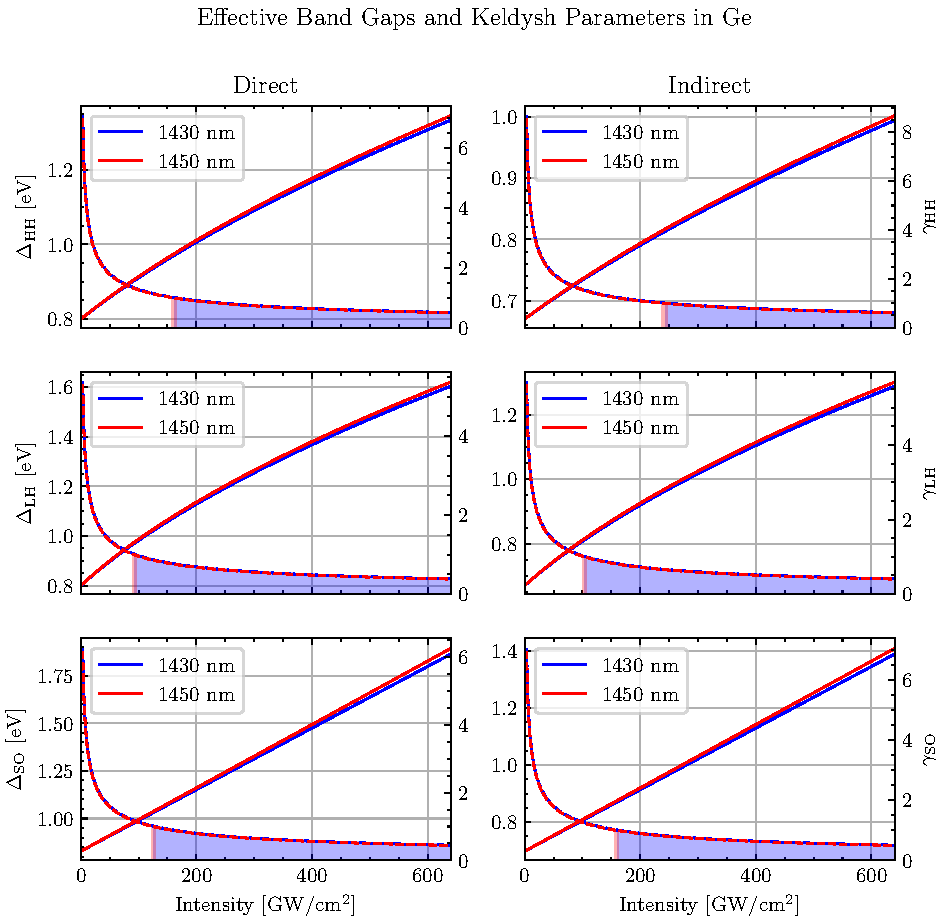
\includegraphics[width=1.0\textwidth]{figures/chap4/Gamma_Gap_Channel_VB_resolved.pdf}
	\caption{Channel- and initial band-resolved effective bandgaps $\Delta_i$ (solid line, left axes) and Keldysh parameters $\gamma_i$ (dashed lines, right axes) as a function of peak intensity. The shaded region under $\gamma_i$ corresponds to intensities where $\gamma_i < 1$ for 1430 nm (blue) and 1450 nm (red).}
	\label{fig:Gamma_Gap_Channel_VB_resolved}
	% plot made with \Python Scripts\DrakeIonization\DrakeIonization.py
\end{figure}

\cref{fig:Gamma_Gap_Channel_VB_resolved} shows the effective band gaps and the Keldysh parameter as a function of peak intensity. The effective bandgap (solid lines, values on left axes) is significant for all initial states and transition types. For example, for a peak intensity of 640 GW/cm\textsuperscript{2} and $\lambda = 1430 \ \textrm{nm}$, the energy required to excite from the light hole band to the conduction band via a direct transition is $\simeq 1.6 \ \textrm{eV}$, which is double the ground state value of 0.8 eV. The dashed lines (values shown on right axis) show the Keldysh parameter $\gamma_i$ for each wavelength. Since $\gamma_i \propto \omega$, the difference between $\gamma_i$ for the two wavelengths is neglible at this scale (about 1.5\%). The shaded region under each $\gamma_i$ curve denotes the intensities at which $\gamma_i<1$. Most intensities resuilt in $\gamma < 1$ or $\gamma \simeq 1$, meaning that both tunnel ionization and multiphoton ionization play an important role. By 250 GW/cm\textsuperscript{2}, $\gamma < 1$ for all possible ionization channels.

%Finally, we convert the excited carrier density to a fractional excitation. Germanium has $N_{\text{u.c.}}=2$ valence electrons per unit cell, and each unit cell has a volume $V_{\text{u.c.}}=4.527 \times 10^{-23} \text{ cm}^{3}$. Therefore the fractional carrier excitation is
%\begin{equation}
%\eta = \Delta N \frac{V_{\text{u.c.}}}{N_{\text{u.c.}}}
%\end{equation}
% NOTE: THIS CONVERSION FACTOR IS WRONG!

% below are the Keldysh ionization rate equations (omitted)
%\begin{equation}
%W_i = \frac{2 \omega}{9 \pi^2} \left( \frac{1}{B} \frac{m \omega}{\hbar} \right)^{3/2} Q\left( \gamma, \frac{\Delta_i^{\textrm{eff}}}{\hbar \omega} \right) \exp \left\{ -\pi \left\langle  \frac{\Delta_i^{\textrm{eff}}}{\hbar \omega} + 1 \right\rangle \times \frac{K(B) - E(B)}{E(A)} \right\}
%\end{equation}
%where we have introduced the shorthand notation:
%\begin{equation}
%\begin{aligned}
%A &= \frac{1}{\sqrt{1+\gamma^2}} \\
%B &= \frac{\gamma}{\sqrt{1+\gamma^2}}
%\end{aligned}
%\end{equation}
%and the function $Q$ is defined as:
%\begin{equation}
%\begin{aligned}
%Q(\gamma, x) &= \left[\pi / 2K(A)\right]^{1/2} \times \sum_{n=0}^{\infty} \left\{-\pi \left[K(B)-E(B)\right] n / E(A) \right\} \\
%&\times \Phi \left\{ \left[\pi^2 \left(2 \langle x+1 \rangle - 2x+n\right) / 2K(A) \times E(A) \right]^{1/2} \right\}
%\end{aligned}
%\end{equation}
%amd the function $\Phi$ is defined as:
%\begin{equation}
%\Phi (z) = ?
%\end{equation}

\subsection{Indirect Transitions}
\label{sec:indirect_transitions}

\begin{figure}
	\centering
	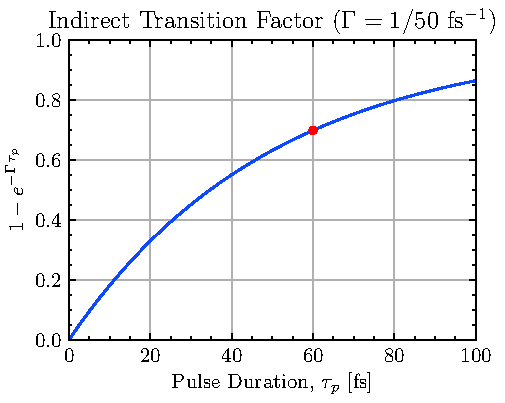
\includegraphics[width=0.75\textwidth]{figures/chap4/Indirect_transition_factor.pdf}
	\caption{Prefactor for indirect transition rates assuming a Poisson distribution. For germanium and a pulse duration of 60 fs, the indirect transition factor is about 0.7. \textbf{NEED TO UPDATE THIS FIGURE WITH NEW PULSE DURATIONS}}
	\label{fig:Indirect_transition_factor}
	% plot made with \Python Scripts\DrakeIonization\DrakeIonization.py
\end{figure}

An indirect transition, where the final crystal momentum is substantially different than its initial value, is mediated by an electron-phonon scattering process. This additional process must occur within the timescale of the laser pulse, and thus we expect the pulse duration and the scattering cross section to impact the relative prevalence of indirect transitions in our experiments. If we assume these collisions occur independent of one another (and, therefore, follow a Poisson distribution), we can calculate the indirect transition ionization rate $W_i^{\textrm{ind.}}$ by multiplying the direct transition rate $W_i^{\textrm{dir.}}$ by a correction factor:
\begin{equation}
W_i^{\textrm{ind.}} = W_i^{\textrm{dir.}} * (1 - \exp(-\Gamma \tau_p))
\label{eqn:Indirect_transition_factor}
\end{equation}
where $\tau_p$ is the pulse duration (\textbf{FWHM OR GUASSIAN PULSE DURATION?}) and $\Gamma$ is the electron-phonon collision rate. The factor in \cref{eqn:Indirect_transition_factor} represents the probability that any given electron will undergo one or more phonon collisions in the time $\tau_p$, assuming the collisions follow a Poisson distribution. For germanium, we estimate $1/\Gamma \approx 47 \ \textrm{fs}$, which is a ballpark figure inferred from measurements of laser-induced periodic surface structures on Ge \cite{austinSemiconductorSurfaceModification2017}. When calculating $W_i^{\textrm{dir.}}$, we use the the local conduction band mass $m_{\textrm{CB}}$ in the indirect valley and the indirect energy gap $\Delta_i^{\textrm{ind.}}$. \cref{fig:Indirect_transition_factor} shows the prefactor in \cref{eqn:Indirect_transition_factor} as a function of pulse duration. \textbf{For our experiment, $\tau_p = 60 \ \textrm{fs}$ and the prefactor evaluates to $\sim 0.72$.} We note that a shorter pulse duration of $\sim 12 \ \textrm{fs}$, which is achievable with our lab's fiber compressor \cite{zhangAtomicMolecularDynamics2015}, would give a prefactor of $\sim 0.23$.

\subsection{Spectral Content of the Laser Pulse}
\label{sec:bandwidth_of_pulse}

\begin{figure}
	\centering
	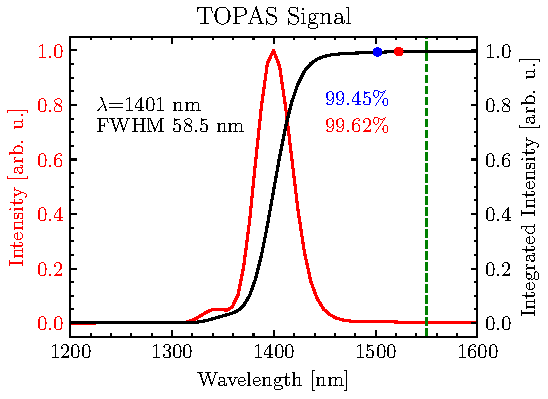
\includegraphics[width=0.75\textwidth]{figures/chap4/TOPAS_1400nm_spectral_inten.pdf}
	\caption{TOPAS spectral content at $\lambda = 1401 \ \textrm{nm}$.}
	\label{fig:TOPAS_1400nm_spectral_inten}
	% figure made in \Python Scripts\FROG\FROG2.py
\end{figure}

Since we are near the bandgap ($\Delta^{\textrm{dir.}} = 1550 \ \textrm{nm}$, $\Delta^{\textrm{ind.}} = 1879 \ \textrm{nm}$), it's possible that a portion of the IR pulse's spectrum will be below the bandgap, which would have consequences for both the interference and Keldysh calculations. \cref{fig:TOPAS_1400nm_spectral_inten} shows the spectral content of the TOPAS when it is set to 1400 nm.\footnote{Unfortunately, we did not measure the spectral content of the pulse when the TOPAS was set at $\lambda = 1430$ or 1450 nm. However, in our experience the shape of the spectral envelope is invariant under small wavelength shifts.} We will use this spectrum to estimate the spectral content when operating at 1430 and 1450 nm. The red line shows the spectral intensity, the black line is the integrated sum of the red line, and the green dashed vertical line represents the direct bandgap. When the TOPAS is operating at 1430 nm (1450 nm), the central wavelength $\lambda_0$ is 120 nm (100 nm) above the bandgap. According to this measurement, when the TOPAS is running at 1400 nm, 99.45\% of the pulse energy is at wavelengths below the $\lambda_0 + 100 \ \textrm{nm}$ (blue dot), and 99.62\% of the pulse energy is at wavelengths below $\lambda_0 + 120 \ \textrm{nm}$ (red dot). If we assume the spectral envelope is invariant under small wavelength shifts, then it stands to reason that when the TOPAS is run at 1430 or 1450 nm, over 99\% of the pulse energy is above Ge's bandgap (1550 nm). Thus, we are justified in treating the pulse as if it were entirely above the band gap.

\subsection{Keldysh Results}
\label{sec:nonlinear_excitation_results}

We now present the ionization results of the model introduced in \cref{sec:nonlinear_excitation_model_details,sec:indirect_transitions}. We start with single-intensity calculations (i.e., what we would observe if we had a $\delta$-function intensity distribution in \cref{fig:TMM_hist_chrom_int_2x2}), then proceed to focal volume average the results using the IR intensity distributions in \cref{sec:thin_film_interference} and \cref{fig:pump_on_focus_calculation}. Focal volume-averaged results are presented in \cref{sec:volume_averaging}.

The simulation was performed for two wavelengths ($\lambda = 1430, 1450 \ \textrm{nm}$) and 1000 different peak intensities, ranging from 3.26 to 640 GW/cm\textsuperscript{2}. A Gaussian pulse envelope was assumed with a pulse duration of $\tau_p = 60 \ \textrm{fs}$, and the time relative to the center of the pulse $\tau$ ranged from -120 to +120 fs in 1000 steps. For each set of input parameters, the simulation outputs an initial band- (HH, LH, SO) and transition type- (indirect, direct) resolved electron population in the conduction band as a function of $\tau$.

\begin{figure}
	\centering
	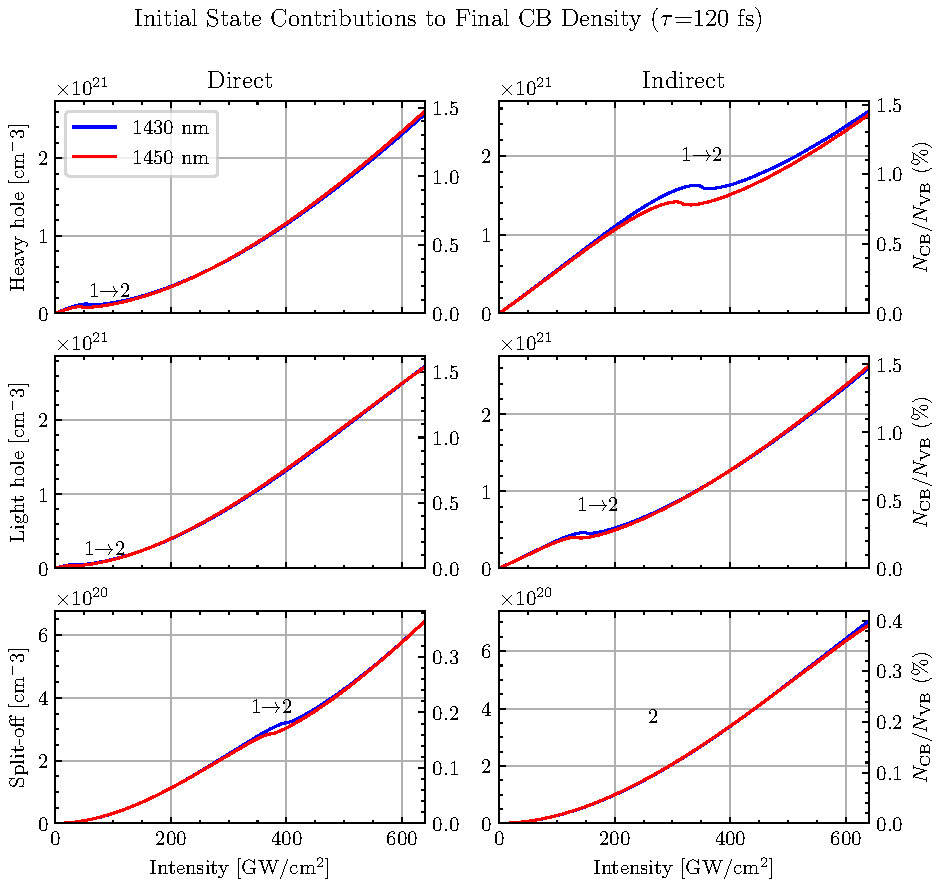
\includegraphics[width=1.0\textwidth]{figures/chap4/N_Channel_VB_resolved.pdf}
	\caption{Transition type and initial band resolved contributions to the final conduction band density. Inset text denotes the values of $n_i$ at the peak intensity (for $\tau=0$ fs) as the minimum number of photons required to excite the electron across the gap increases by 1.}
	\label{fig:N_Channel_VB_resolved}
	% plot made with \Python Scripts\DrakeIonization\DrakeIonization.py
\end{figure}

\cref{fig:N_Channel_VB_resolved} shows the main result of the Keldysh calculation. We plot the contributions from each ionization channel (direct \& indirect) and for each of the three initial bands after the IR pulse has left ($\tau = 120 \ \textrm{fs}$) as a function of peak intensity. We see an intensity-dependent effect where $N_{\textrm{CB}}$ has a local maximum, a slight dip, and then an increase. At this scale, this feature is most prominent in for indirect heavy hole plot, but the general shape is the same for all channels. These features occur at intensities that coincide with an increase in the minimum number of photons required to cross the bandgap ($n_i$ in \cref{eqn:min_number_photons}), akin to channel-closure \cite{shcheblanovNonlinearPhotoionizationTransparent2017}. The value of $n_i$ is denoted in the plot on either side of the feature.
%We interpret this as a result of the effective bandgap changing with increasing field strength (see \cref{eqn:eff_bandgap_HHLL,eqn:eff_bandgap_SO}).

\begin{figure}
	\centering
	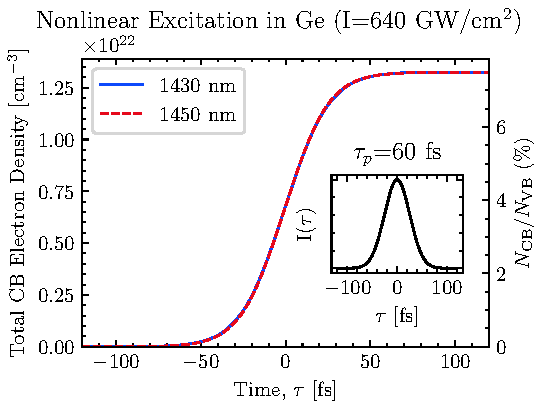
\includegraphics[width=0.75\textwidth]{figures/chap4/Total_CB_dens_vs_Time.pdf}
	\caption{Total valence band (VB) population as a function of laser pulse delay. Inset shows the pulse envelope.}
	\label{fig:Total_CB_dens_vs_Time}
	% plot made with \Python Scripts\DrakeIonization\DrakeIonization.py
\end{figure}

\cref{fig:Total_CB_dens_vs_Time} shows the total excitation (summed over all channels and initial bands) of the sample as a function of $\tau$ for the highest intensity ($I = 640$ GW/\textsuperscript{2}). The result is a modified error function, owing to the nonlinearity of the sample's response. We see there is little difference between the two wavelengths in terms of total excitation. Because we use the pulse envelope, rather than the instantenous field strength, we do not see steps in the ionization fraction every half-period \cite{schultzeAttosecondBandgapDynamics2014}.

\begin{figure}
	\centering
	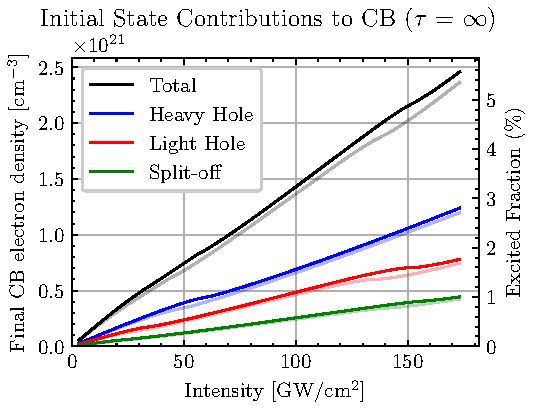
\includegraphics[width=0.75\textwidth]{figures/chap4/CB_dens_vs_Int.pdf}
	\caption{Contributions of the initial bands to the final conduction band (CB) density at the end of the pulse ($\tau = \infty$). Dark lines are for $\lambda = 1430 \ \textrm{nm}$, faint lines are for $\lambda = 1450 \ \textrm{nm}$.}
	\label{fig:CB_dens_vs_Int}
	% plot made with \Python Scripts\DrakeIonization\DrakeIonization.py
\end{figure}

\cref{fig:CB_dens_vs_Int} shows the population of the conduction band after the IR pulse has left (${\tau = 120 \ \textrm{fs}}$) as a function of peak intensity. For all intensities, the signal is dominated by contributions by the heavy and light holes, which is to be expected as the split-off band has a higher ionization potential. For 1430 nm, we see that at 160 GW/cm\textsuperscript{2}, the heavy hole VB is responsible for about 50.2\% of the CB population, followed by the light hole VB at around 31.8\%, and finally the split-off VB at around 18.0\% percent, with similar ratios for 1450 nm. Above 400 GW/cm\textsuperscript{2}, the LH contribution begins to overtake the HH. In our experience, a peak intensity of above 640 GW/cm\textsuperscript{2} corresponds to immediate sample damage, meaning that we can expect no more than $1.32 \times 10^{22} \textrm{cm}^{-3} \simeq 7.5\% \ N_{\textrm{VB}}$ fractional excitation in our experiments. This indicates that ultrafast melting should not be a concern below 640 GW/cm\textsuperscript{2}.

\begin{figure}
	\centering
	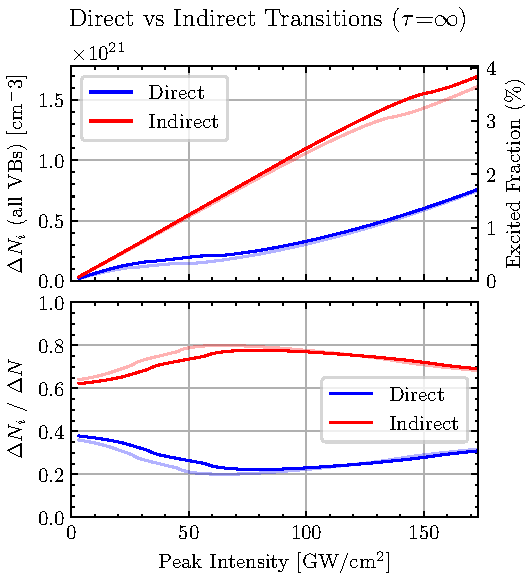
\includegraphics[width=0.75\textwidth]{figures/chap4/Direct_vs_Indirect_Trans.pdf}
	\caption{Contributions by indirect and direct transitions to the final conduction band (CB) density at the end of the pulse ($\tau = \infty$). Dark lines are for $\lambda = 1430 \ \textrm{nm}$, faint lines are for $\lambda = 1450 \ \textrm{nm}$.}
	\label{fig:Direct_vs_Indirect_Trans}
	% plot made with \Python Scripts\DrakeIonization\DrakeIonization.py
\end{figure}

\cref{fig:Direct_vs_Indirect_Trans} shows the relative contribution of indirect and direct transitions to the total population density by the end of the pulse as a function of peak intensity. Recalling \cref{eqn:Indirect_transition_factor}, the indirect transition rate is suppressed due to the product $\tau_p \Gamma \approx 0.7$. However, this factor is not enough to overcome the relative increase in ionization due to the lower bandgap of the indirect transition compared to the direct transition. Consequently, only {20 - 50\%} of the excited population are due to direct transitions. At the highest intensities, we see equal contributions by both channels.

\textbf{question}: which electron populations are we sensitive to in our measurement?

The above calculations assume a single peak intensity throughout the sample, but a spatially invariant intensity profile is unphysical. In a real experiment, the sample experiences a spatially varying intensity profile, which results in a nonuniform excitation fraction. We have already addressed the diffraction-induced transverse intensity profile of the IR focus (see \cref{sec:Pump_Arm_Focus_Calculations}). In the following section, we will calculate the intensity profile along the direction of propagation within the sample.

\subsection{Thin Film Interference Calculations}
\label{sec:thin_film_interference}

%\begin{figure}
%	\centering
%	\subfloat[]{
%		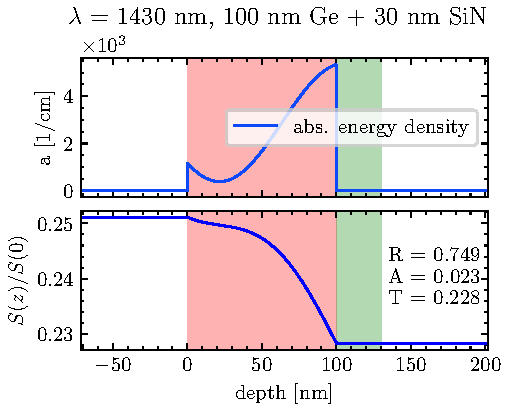
\includegraphics[width=0.75\textwidth]{figures/chap4/GeSiN_RAT_1430nm.pdf}
%		\label{fig:GeSiN_RAT_1430nm}}
%	
%	\subfloat[]{
%		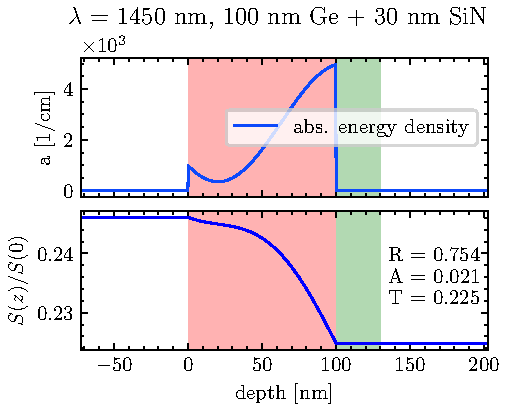
\includegraphics[width=0.75\textwidth]{figures/chap4/GeSiN_RAT_1450nm.pdf}
%		\label{fig:GeSiN_RAT_1450nm}}
%	\caption{Thin film calculations for the sample heterostructure for $\lambda = 1430 \ \textrm{nm}$ and $1450 \ \textrm{nm}$. The red region represents germanium; green is silicon nitride; white is vacuum. The top panel shows the absorbed energy density per unit input power. The bottom panel shows the local intensity $S(z) \equiv \vb{S}(z) \vdot \hat{z}$, normalized by the input intensity $S(0) \equiv \vb{S}(0) \vdot \hat{z}$. See text for details.}
%	\label{fig:GeSiN_RAT:both}
%	% python script: \Python Scripts\thinfilm\thinfilm.py
%\end{figure}

The sample is a heterostructure of 100 nm germanium ($\tilde{n} = 4.2481 + 0.066041i$ at 1430 nm) on a 30 nm silicon nitride membrane ($\tilde{n}=1.9997 + 0i$ at 1430 nm) with a total thickness measuring $\sim 9$\% of the fundamental wavelength. As a result, we cannot ignore thin film interference effects that may arise from this geometry. To account for this, we calculated the intensity profile in the heterostructure for the two wavelengths of experimental interest (1430 and 1450 nm) using the transfer matrix method. We also calculate the intensity profile with the assumption that there is no internal interference pattern. As will be shown below, these two methods result in drastically different intensity profiles. The actual internal profile is likely somewhere between the two, as the sample is not an ideal thin film, nor is its quality so poor that it is completely incapable of supporting interference patterns. The resulting intensity profiles are later used as inputs to the Keldysh nonlinear photoionization code. Refractive index data for germanium \cite{nunleyOpticalConstantsGermanium2016} and the silicon nitride \cite{lukeBroadbandMidinfraredFrequency2015} were taken from the literature. Calculations were performed using the \textit{TMM package for Python} \cite{byrnesTmmSimulateLight2017,byrnesMultilayerOpticalCalculations2019}.

The TMM code assumes a multilayer planar stack of non-magnetic ($\mu = \mu_0$) and isotropic materials. The interfaces are considered ideal (i.e., zero surface roughness), so this result represents an upper limit on the interference effects present in our system. Nonlinear effects are excluded from this calculation. The electric field is expressed as a superposition of forward- and backward-propagating complex-valued waves:
\begin{equation}
\begin{aligned}
\vb{E}(\vb{r}) &= \vb{E}_f^0 \exp(i \vb{k}_f \vdot \vb{r}) + \vb{E}_b^0 \exp(i \vb{k}_b \vdot \vb{r}), \\
\vb{k}_f &= \frac{2 \pi n}{\lambda_{\textrm{vac}}} \left( \vu{z} \cos \theta + \vu{x} \sin \theta \right), \\
\vb{k}_b &= \frac{2 \pi n}{\lambda_{\textrm{vac}}} \left( - \vu{z} \cos \theta + \vu{x} \sin \theta \right),
\end{aligned}
\end{equation}
where $\theta$ is the angle between $\vb{k}$ and the surface normal. The code solves for the internal complex electric field by applying the transfer matrix method to the heterostructure assuming an input electric field of unit magnitude \cite{nistadCausalityElectromagneticProperties2008,harbeckeCoherentIncoherentReflection1986,ohtaMatrixFormalismCalculation1990,katsidisGeneralTransfermatrixMethod2002,shalabneyElectromagneticFieldsDistribution2010}. We obtain the physical field at any time $t$ by multiplying the complex field by $e^{-i \omega t}$ and taking the real part of the resulting expression. We define the \textit{peak normalized intensity} as the local peak intensity divided by the peak intensity in the absence of the heterostructure\footnote{We omit the denominator as it evaluates to unity with an input field of unit strength. That is, $\textrm{max}_{t}\left( \left|\sum_{\lambda}\vb{E}_{\textrm{vac.},\lambda}\right|^2 \right) = 1$.}:
\begin{equation}
\frac{I_p(z)}{I_{p,0}(z)} \equiv \Re{\tilde{n}_{\lambda_0}(z)} \ \textrm{max}_{t}\left(\left|\sum_{\lambda}\vb{E}_\lambda(z, t)\right|^2 \right)
\end{equation}
where $\tilde{n}_{\lambda_0}(z)$ is complex refractive index at the central wavelength at position $z$. The normalized peak intensity will later be used to convert vacuum intensities to sample intensities. We also report the transmitted ($T$), reflected ($R$) and absorbed power ($A$) of the heterostructure.

\begin{figure}
	\centering
	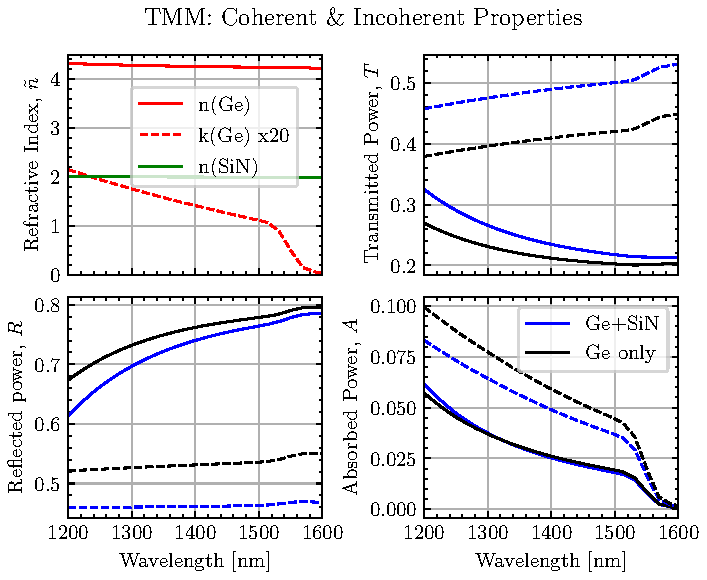
\includegraphics[width=0.9\textwidth]{figures/chap4/tmm_vs_WL_1200-1600nm.pdf}
	\caption{Optical properties of the Ge/SiN heterostructure and a freestanding 100 nm Ge membrane as a function of wavelength. For the $R$, $A$ and $T$ panels, solid lines represent the coherent calculations, and dashed lines represent the incoherent calculations. TMM calculations assume monochromatic light.}
	\label{fig:tmm_vs_WL_1200-1600nm}
\end{figure}

We start by considering the wavelength dependence of the calculated optical properties. The top left panel of \cref{fig:tmm_vs_WL_1200-1600nm} shows the complex refractive index of germanium and silicon nitride over the range 1200 -- 1600 nm. Note that the vertical scale for k(Ge) has been enlarged for visual clarity. In the following discussion, we consider either a heterostructure (germanium sample at {$z$ = 0 -- 100 nm}, silicon nitride at {$z$ = 100 -- 130 nm}, and vacuum elsewhere) or a freestanding germanium film (germanium sample at {$z$ = 0 -- 100 nm}, and vacuum elsewhere). The IR laser propagates in the $+z$ direction with a normal incidence angle ($\theta = 0$). The refractive index for silicon nitride is effectively constant over this range, and germanium's index is well-behaved below 1520 nm (near the direct bandgap at 1550 nm). The solid lines in the remaining three panels of \cref{fig:tmm_vs_WL_1200-1600nm} show the transmitted, reflected and absorbed power for both a freestanding 100 nm Ge film and a 100 nm Ge / 30 nm SiN hetereostructure assuming full coherence of the beam. The dashed lines in these panels show the results of an \textit{incoherent TMM calculation}, in which we discard the phase information of the light to approximate the effects of a rough surface or spatially varying film thickness.

As should be expected, interference effects are critical to understanding the optical properties when the structure is sub-wavelength. The coherence is responsible for nearly doubling the reflectance and reducing the absorbed power by a factor of $\approx 2.5$ at 1400 nm.  We can see that the reflected and transmitted power do not change appreciably over the range {1400 -- 1500 nm}, which encompasses the spectral envelope of a TOPAS signal centered at 1430 or 1450 nm. For both the hetereostructure and the freestanding Ge film, about 75 percent of the incident power is reflected, about 23 percent is transmitted, and about 2 percent is linearly absorbed.

We note that at these wavelengths the coherence length, $L$, greatly exceeds the sample thickness \cite{katsidisGeneralTransfermatrixMethod2002}:
\begin{equation}
L = \frac{\lambda^2}{n \Delta \lambda}
\end{equation}
For a laser pulse with a central wavelength of 1430 nm and a bandwidth of 58.5 nm, $L(\textrm{Ge}) \approx 8.23 \ \mu\textrm{m}$ and $L(\textrm{SiN}) \approx 17.4 \ \mu\textrm{m}$, which is $\approx 80$ and $\approx 580$ times longer than the thickness of the germanium and silicon nitride films, respectively. We also note that a round trip reflection within the heterostructure will take 3.2 fs at 1430 nm, which is 18 times shorter than the laser pulse. For these reasons, we use standard interference calculation methods to estimate the intensity profile within the heterostructure.
%Additionally, we can quantify the effect of the SiN membrane, which was required due to the technical limitations of our sample preparation process.

%We also report the normalized absorbed energy density, $a(z)$:
%\begin{equation}
%a(z) = \frac{\left|E_f + E_b \right|^2 \Im \left[n \cos(\theta) k_z\right]}{\Re \left[ n_0 \cos \theta_0 \right]},
%\end{equation}
%where the zero subscript denotes the quantity in vacuum. We also calculate the peak normalized intensity, $I_p(z) / I_{p,0}(z)$, which is the local peak intensity divided by the peak intensity in the absence of the heterostructure. The transmitted ($T$), reflected ($R$) and absorbed power ($A$) of the heterostructure are also reported. 
%For $s$-polarized light, the normal component of the Poynting vector $\vb{S} \vdot \vu{z}$ at position $z$ can be written as:
%\begin{equation}
%S(z) \equiv \vb{S} \vdot \vu{z} = \frac{1}{2} \Re \left[ \vu{z} \vdot (\vb{E^*} \cp \vb{H}) \right] \ \propto \Re \left[ (E_f^* + E_b^*)(E_f-E_b) n \cos \theta \right],
%\end{equation}
%where $E_f$ ($E_b$) is the forward (backward) amplitude evaluated at position $z$. We report this quantity normalized by the normal component of the incident Poynting vector that would result from the absence of the heterostructure ($\vb{S} \vdot \vu{z}$  with $E_b = 0$ and $E_f = 1$):
%\begin{equation}
%\frac{S(z)}{S(0)} = \frac{\Re \left[ (E_f^* + E_b^*)(E_f-E_b) n \cos \theta \right]}{\Re \left[n_0 \cos \theta_0 \right]},
%\end{equation}
%where the zero subscript denotes the quantity in vacuum.
%\begin{figure}
%	\centering
%	\subfloat[]{
%		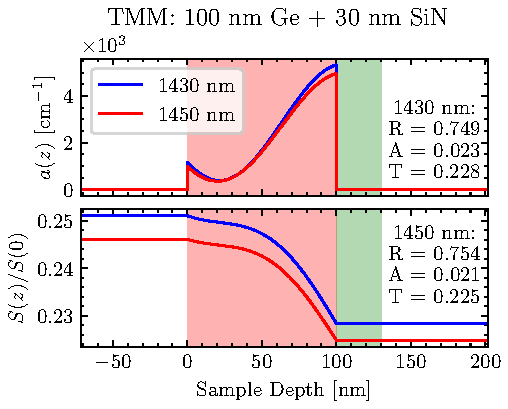
\includegraphics[width=0.75\textwidth]{figures/chap4/TMM_1430_1450_RAT.pdf}
%		\label{fig:TMM_1430_1450_RAT}}
%	
%	\subfloat[]{
%		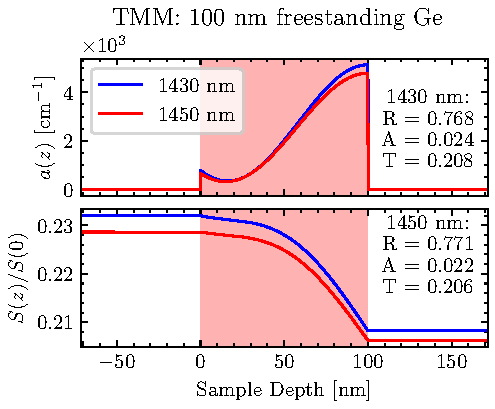
\includegraphics[width=0.75\textwidth]{figures/chap4/TMM_1430_1450_Geonly_RAT.pdf}
%		\label{fig:TMM_1430_1450_Geonly_RAT}}
%	\caption{Thin film calculations at $\lambda = 1430 \ \textrm{nm}$ and $1450 \ \textrm{nm}$ for (a): {100 nm} Ge film on a {30 nm} SiN membrane and (b): {100 nm} freestanding Ge membrane. The red region represents germanium; green is silicon nitride; white is vacuum. See text for details.}
%	\label{fig:GeSiN_RAT:both}
%	% python script: \Python Scripts\thinfilm\thinfilm.py
%\end{figure}
\begin{figure}
	\centering
	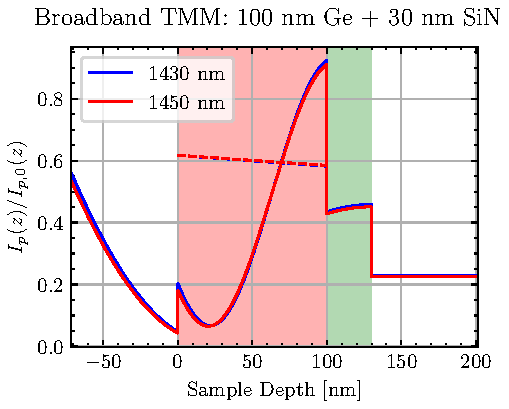
\includegraphics[width=0.75\textwidth]{figures/chap4/TMM_1430_1450_broad_Int.pdf}
	\caption{Broadband TMM calculations for a {100 nm} Ge film and {30 nm} SiN membrane. The red region represents Ge; green is SiN; white is vacuum. Solid lines are TMM results, dashed lines are \cref{eqn:Iint_fresnel_losses}.}
	\label{fig:TMM_1430_1450_broad_Int}
	% python script: \Python Scripts\thinfilm\thinfilm.py
\end{figure}
%\begin{figure}
%	\centering
%	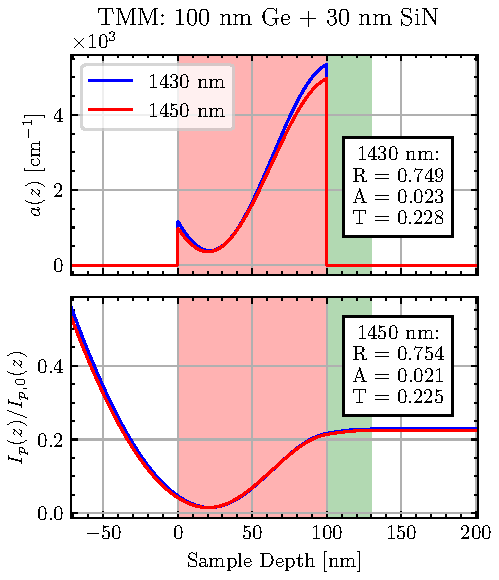
\includegraphics[width=0.75\textwidth]{figures/chap4/TMM_1430_1450_RAT_a_Int.pdf}
%	\caption{TMM calculations for a {100 nm} Ge film and {30 nm} SiN membrane. The red region represents Ge; green is SiN; white is vacuum. See text for details.}
%	\label{fig:TMM_1430_1450_RAT_a_Int}
%	% python script: \Python Scripts\thinfilm\thinfilm.py
%\end{figure}
%\begin{figure}
%	\centering
%	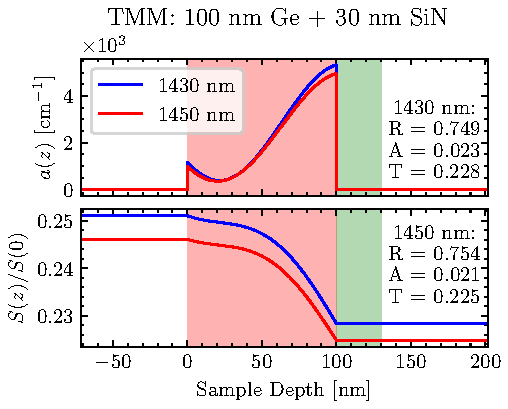
\includegraphics[width=0.75\textwidth]{figures/chap4/TMM_1430_1450_RAT.pdf}
%	\caption{Thin film calculations for the sample heterostructure for $\lambda = 1430 \ \textrm{nm}$ and $1450 \ \textrm{nm}$. The red region represents germanium; green is silicon nitride; white is vacuum. The top panel shows the absorbed energy density per unit input power. The bottom panel shows the normal component of the Poynting vector, normalized by the incident intensity. See text for details.}
%	\label{fig:TMM_1430_1450_RAT}
%	% python script: \Python Scripts\thinfilm\thinfilm.py
%\end{figure}

Since the TMM model is linear, we can extend it to handle a broadband pulse by coherently summing the resulting electric field over the bandwidth of the pulse. Broadband TMM calculations were performed using $N=500$ monochromatic TMM calculations over the spectral range 1300 - 1500 nm. Spectral weights for each wavelength were calculated by interpolating the square root of the spectral intensity in \cref{fig:TOPAS_1400nm_spectral_inten} after shifting the spectral envelope to the appropriate central wavelength.

We compare the TMM result to a simpler model which only includes Fresnel losses from the front interface (vacuum-Ge) and linear absorption thereafter \cite{zurchDirectSimultaneousObservation2017}:
\begin{equation}
\frac{I_p(z)}{I_{p,0}(z)} = \Re{\tilde{n}} \left| \frac{2}{1+\tilde{n}} \right|^2 \exp \left[ - \left( \frac{4 \pi}{\lambda_0} \right) \Im{\tilde{n}} z \right] \approx 0.60,
\label{eqn:Iint_fresnel_losses}
\end{equation}
where $\tilde{n}$ is the complex refractive index of Ge evaluated at the central wavelength of the pulse ($\lambda_0$) and $z$ is the depth within the Ge sample. While this method does not calculate the intensity profile outside of the germanium, we note that this information is superfluous as SiN's large band gap ($\Delta \approx 5 \ \textrm{eV}$) precludes any linear absorption, and our XUV measurement is insensitive to any dynamics occuring within the SiN membrane.

\cref{fig:TMM_1430_1450_broad_Int} shows the calculated peak normalized intensity profile of a heterostructure consisting of 100 nm of germanium on a 30 nm thick silicon nitride membrane for $\lambda = 1430$ and 1450 nm. The solid lines are broadband TMM calculations, and the dashed lines are the Fresnel absorption model (\cref{eqn:Iint_fresnel_losses}). Starting with the TMM result, we note that the discrete jumps in intensity at the sample boundaries are due to the discrete jumps in the refractive index. Inside the Ge, we see a strong modulation of the intensity due to interference effects. Before the sample ($z < 0$), the intensity is suppressed by the coherent back reflection from the vacuum-Ge interface. Inside the sample, the intensity has a minimum about 20 nm below the vacuum-Ge interface. From $z=20 \ \textrm{nm}$ to $z=80 \ \textrm{nm}$ the normalized peak intensity increases linearly before asymtoptically approaching a maximum value at the Ge-SiN boundary. Therefore, the broadband TMM model predicts that the highest intensities are located on the back face of the Ge sample, which can be understood as a combined reflection off the Ge-SiN and SiN-vacuum interfaces. In contrast to the TMM result, \cref{eqn:Iint_fresnel_losses} yields an intensity profile that is very nearly linear over the limited 100 nm distance. In either model, changing the wavelength from 1430 nm to 1450 nm does not appreciably change the intensity profile.

%\begin{figure}
%	\centering
%	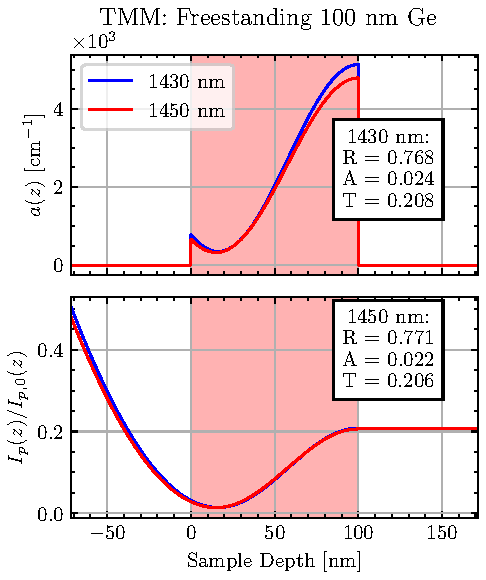
\includegraphics[width=0.75\textwidth]{figures/chap4/GeOnly_1430_1450_RAT_a_Int.pdf}
%	\caption{TMM calculations for a {100 nm} freestanding Ge thin film. The red region represents Ge; white is vacuum. See text for details.}
%	\label{fig:GeOnly_1430_1450_RAT_a_Int}
%	% python script: \Python Scripts\thinfilm\thinfilm.py
%\end{figure}
\begin{figure}
	\centering
	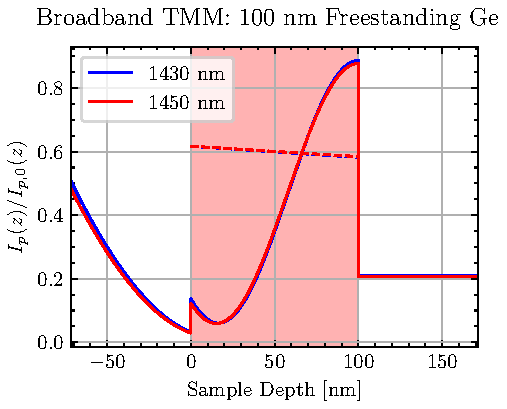
\includegraphics[width=0.75\textwidth]{figures/chap4/Ge_1430_1450_broad_Int.pdf}
	\caption{Broadband TMM calculations for a {100 nm} freestanding Ge thin film. The red region represents Ge; white is vacuum. Solid lines are TMM results, dashed lines are \cref{eqn:Iint_fresnel_losses}.}
	\label{fig:Ge_1430_1450_broad_Int}
	% python script: \Python Scripts\thinfilm\thinfilm.py
\end{figure}

The presence of the silicon nitride membrane was required for technical materials preparation reasons. To quantify the effect of its presence on the internal intensity distribution, we performed broadband TMM calculations for a 100 nm thick freestanding germanium membrane, as shown in \cref{fig:Ge_1430_1450_broad_Int}. Comparing it to the previous result, we can see that the addition of the SiN membrane does not significantly change the optical properties of the sample, as the general shape of the intensity profile is the same as the heterostructure. By adding the SiN membrane, reflectivity increases by $\approx 2.5\%$, absorption decreases by $\approx 4.2\%$, and transmission increases by $\approx 9.6\%$. The increased reflection losses are not a concern, as we have sufficient flux in our pump arm to make up for the increased losses. The dashed lines show \cref{eqn:Iint_fresnel_losses}, which does not take into account the presence or absence of the SiN membrane and is the same as in \cref{fig:TMM_1430_1450_broad_Int}.

If the sample response was strictly linear, then the measured ATAS signal should be proportional to the average intensity within the XUV probe. For the Ge/SiN heterostructure, the average intensity of the TMM model is about 65\% that of the Fresnel model. On the other hand, a nonlinear sample response gives the higher intensity regions outsized importance, and we see that the broadband TMM interference pattern has a maximum intensity 50\% higher than the Fresnel model. These numbers are similar for the freestanding germanium geometry, albeit less pronounced (average intensity TMM:average intensity Frensel = 0.68, maximum intensity TMM:maximum intensity Fresnel = 0.44).

\begin{table}[]
	\centering
	\begin{tabular}{l|l|l|l|l}
		\textbf{TMM Type} &
		\textbf{Structure} &
		\textbf{$\lambda_0$ {[}nm{]}} &
		\textbf{min$\left(\frac{I_p(z)}{I_{p,0}(z)}\right)$ {[}\%{]}} &
		\textbf{max$\left(\frac{I_p(z)}{I_{p,0}(z)}\right)$ {[}\%{]}} \\ \hline
		\multirow{4}{*}{monochromatic} & \multirow{2}{*}{Ge/SiN}          & 1430 & 6.62 & 92.62 \\
		&                                  & 1450 & 6.49 & 91.24\\ \cline{2-5} 
		& \multirow{2}{*}{freestanding Ge} & 1430 & 5.93 & 88.50 \\
		&                                  & 1450 & 5.86 & 87.53 \\ \hline
		\multirow{4}{*}{broadband}     & \multirow{2}{*}{Ge/SiN}          & 1430 & 6.68 & 92.19 \\
		&                                  & 1450 & 6.53 & 90.90 \\ \cline{2-5} 
		& \multirow{2}{*}{freestanding Ge} & 1430 & 6.01 & 88.67 \\
		&                                  & 1450 & 5.90 & 87.84
	\end{tabular}
	\caption{TMM calculated internal intensity ranges for a 100 nm Ge / 30 nm SiN heterostructure and a freestanding Ge film.}
	\label{tab:TMM_intensity_range}
\end{table}
%\begin{table}[]
%	\centering
%	\begin{tabular}{l|l|l|l|l}
%		\textbf{TMM Type} &
%		\textbf{Structure} &
%		\textbf{$\lambda_0$ {[}nm{]}} &
%		\textbf{min$\left(\frac{I_p(z)}{I_{p,0}(z)}\right)$ {[}\%{]}} &
%		\textbf{max$\left(\frac{I_p(z)}{I_{p,0}(z)}\right)$ {[}\%{]}} \\ \hline
%		\multirow{4}{*}{\textbf{monochromatic}} & \multirow{2}{*}{Ge/SiN}          & 1430 & 1.56 & 21.70 \\
%		&                                  & 1450 & 1.53 & 21.40 \\ \cline{2-5} 
%		& \multirow{2}{*}{freestanding Ge} & 1430 & 1.40 & 20.80 \\
%		&                                  & 1450 & 1.38 & 20.60 \\ \hline
%		\multirow{4}{*}{\textbf{broadband}}     & \multirow{2}{*}{Ge/SiN}          & 1430 & 1.57 & 21.60 \\
%		&                                  & 1450 & 1.54 & 21.32 \\ \cline{2-5} 
%		& \multirow{2}{*}{freestanding Ge} & 1430 & 1.42 & 20.84 \\
%		&                                  & 1450 & 1.39 & 20.65
%	\end{tabular}
%	\caption{TMM calculated internal intensity ranges for a 100 nm Ge / 30 nm SiN heterostructure and a freestanding Ge film. See text for details.}
%	\label{tab:TMM_intensity_range}
%\end{table}

A simple monochromatic TMM calculation at the central wavelength of the pulse can reveal much of the same information in a fraction of the computational time. \cref{tab:TMM_intensity_range} shows intensity extrema for the different sample geometries, wavelengths and TMM calculation methods. For our relatively narrow bandwidth, including the coherent sum over all wavelengths changes the results by about 1\%. Not shown are the monochromatic versions of \cref{fig:TMM_1430_1450_broad_Int,fig:Ge_1430_1450_broad_Int}, but the differences between the two methods are imperceptible at this scale.

\begin{figure}
	\centering
	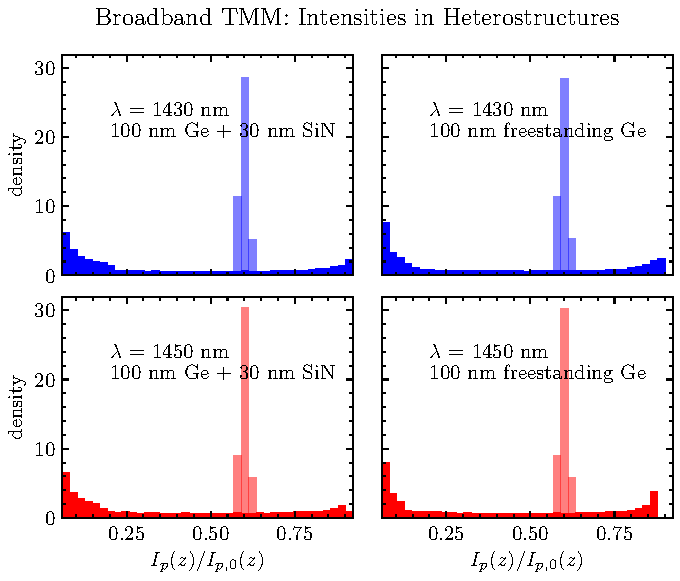
\includegraphics[width=0.75\textwidth]{figures/chap4/TMM_hist_chrom_int_2x2.pdf}
	\caption{Calculated intensity distributions in Ge/SiN heterostructures and Ge thin films. Dark colors follow broadband TMM calculations, light colors follow \cref{eqn:Iint_fresnel_losses}.}
	\label{fig:TMM_hist_chrom_int_2x2}
	% python script: \Python Scripts\thinfilm\thinfilm.py
\end{figure}

The distribution of intensities within the sample is important when calculating the focal volume averaged Keldysh ionization, and anything short of a $\delta$-function distribution of intensities will smear out intensity-dependent effects. \cref{fig:TMM_hist_chrom_int_2x2} shows histograms ($N = 40$ bins) of the intensity distributions of the aforementioned sample geometries and experimental conditions. The dark colors are the results of the broadband TMM calculation, and the lighter colors follow from \cref{eqn:Iint_fresnel_losses}. The general shape of the TMM's distribution is similar for both wavelengths and sample geometries. In all four cases, most of the sample sees relatively low intensities ($<20\%$ of the incident intensity), whereas on the volume closest to the rear face of the stack experiences high intensities ($>75\%$ of the incident intensity). The distribution is flat for intermediate intensities ({20 -- 75 \%} of the incident intensity), owing to the linear increase of intensity with increasing $z$. It should be noted that the high-intensity tail of the freestanding Ge samples is slightly more pronounced than the Ge/SiN heterostructures, which could facilitate the measurement of intensity-dependent effects. In contrast, the Fresnel absorption model (\cref{eqn:Iint_fresnel_losses}) predicts a near-$\delta$ function intensity distribution.

These calculations were run over a range of incident angles. The resulting intensity distribution does not appreciably change for either s- or p-polarized light if the incident angle remains below 20 degrees (measured from normal). We did not carefully control for the incident angle when installing our samples, but since this result is not sensitive to the incident angle, it is reasonable to assume that our sample experiences the intensity distribution shown in \cref{fig:TMM_hist_chrom_int_2x2}.
%for TMM results vs. incident angle, see the code block at end of thinfilm.py. I did not save these results to disk.

Having computed the intensity profile within the Ge sample, we can now apply the Keldysh model to our experiment.

\subsection{Volume Averaging}
\label{sec:volume_averaging}

We calculate the intensity inside the sample as the product of the sample-free vacuum intensity $I_{\textrm{vac.}}$, the transverse diffraction-induced term $I_{\textrm{diff.}}(x, y)$ (\cref{fig:pump_on_focus_calculation}) and the interference/absorption term $I_p(z) / I_{p,0}(z)$ (\cref{sec:thin_film_interference}):

\begin{equation}
I_{\textrm{sample}}(x, y, z, \tau) \equiv I_{\textrm{vac.}}(\tau) \times I_{\textrm{diff.}}(x, y) \times \frac{I_p(z)}{I_{p,0}(z)}
\label{eqn:sample_intensity_XYZtau}
\end{equation}

We provide a brief summary of the aforementioned profiles here. Combining the first two terms, $I_{\textrm{vac.}} \times I_{\textrm{diff.}}$ has a peak intensity at the focus of $\approx 2.3 \times 10^{11}$ W/cm\textsuperscript{2} per 1 $\mu$J input energy (as measured before lens L4), and $I_p(z) / I_{p,0}(z)$ has a maximum value of about 93\% (for a Ge/SiN heterostructure). Therefore, the maximum peak intensity in the germanium sample is approximately $2.13 \times 10^{11}$ W/cm\textsuperscript{2} per 1 $\mu$J input energy. 

\begin{figure}
	\centering
	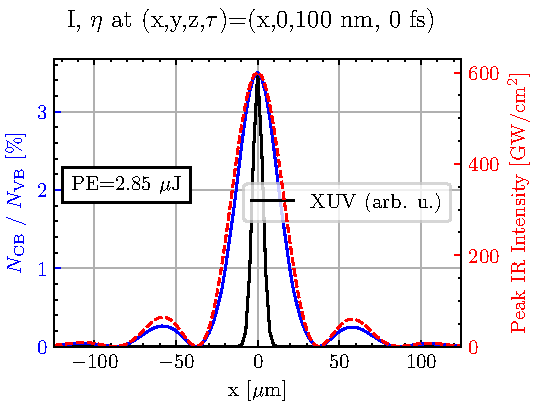
\includegraphics[width=0.75\textwidth]{figures/chap4/excitation_at_focus.pdf}
	\caption{Cross sectional slice of the IR intensity profile, XUV intensity profile and total excited state fraction at the rear of the Ge sample in a Ge/SiN heterostructure and the center of the IR pulse ($\tau = 0 \ \textrm{fs}$). The IR intensity profile follows from a broadband TMM calculation for a 100 nm Ge / 30 nm SiN hetereostructure and an input pulse energy of 2.85 $\mu$J of $\lambda = 1430 \ \textrm{nm}$.}
	\label{fig:excitation_at_focus}
	% plot made with \Python Scripts\DrakeIonization\VolumeAveraging_class_script.py
\end{figure}

We map the Keldysh simulation result $N_{\textrm{CB}}(I, \tau)$ onto the intensity distribution $I_{\textrm{sample}}(x, y, z, \tau)$ to get the conduction band electron density distribution $N_{\textrm{CB}}(x, y, z, \tau)$ within the sample. \cref{fig:excitation_at_focus} shows an example lineout of the IR intensity and the conduction band electron density in our sample. This slice was taken at the Ge/SiN interface ($z=100$ nm) at the peak of the pulse ($\tau=0$ fs), where the intensity is the highest. We see that the excitation (blue solid line) mostly follows the Airy-like diffraction pattern of the IR intensity (red dashed line). Deviations between the two profiles are due to the nonlinear response of the sample to the laser. The XUV profile is also shown (black solid line) in arbitrary units, which will be used to perform the volume averaging integral, \cref{eqn:Delta_A_3}.

\begin{figure}
	\centering
	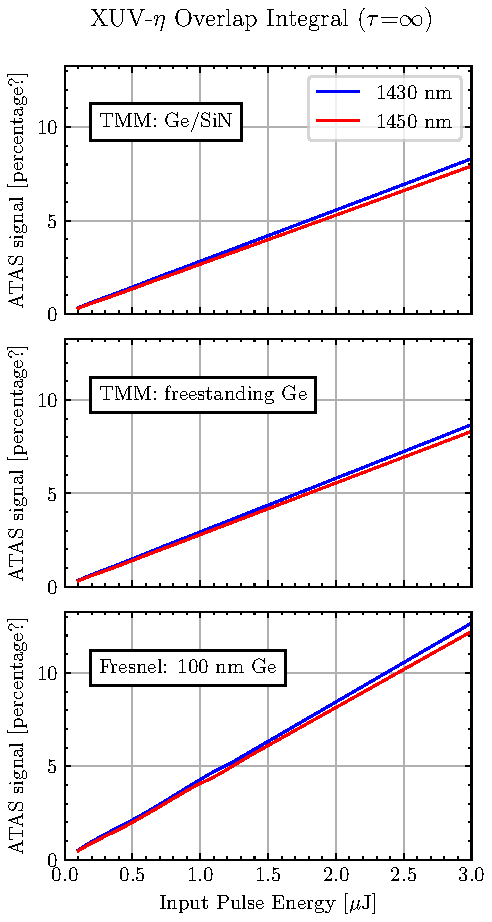
\includegraphics[width=0.75\textwidth]{figures/chap4/FVA_XUV_signal.pdf}
	\caption{Calculated final $\Delta A$ as a function of input pulse energy. These curves were calculated using $\alpha_{10}(32 \ \textrm{eV})$ (absorption).}
	\label{fig:FVA_XUV_signal}
	% plot made with \Python Scripts\DrakeIonization\VolumeAveraging_class_script.py
\end{figure}

\cref{fig:FVA_XUV_signal} shows the intensity scaling of the focal volume averaged $\Delta A$ for the three different intensity profiles. There is little difference between the Ge/SiN heterostructure and freestanding results, which follows from their simliar internal intensity profiles. This confirms our suspiscion that the SiN membrane does not strongly affect the experimental results. On the contrary, the simple Fresnel absorption model has a narrow intensity distribution, and as a result the intensity-dependent features persist through the volume averaging. The higher average intensity of the Fresnel absorption model results in a signal that is about 40\% higher than either TMM intensity distribution.

\begin{figure}
	\centering
	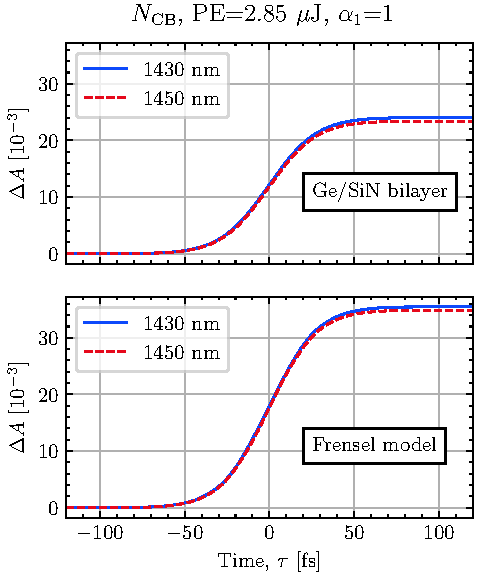
\includegraphics[width=0.75\textwidth]{figures/chap4/FVA_Total_CB_dens_vs_T.pdf}
	\caption{Calculated $\Delta A$ as a function of pulse delay time, $\tau$. These curves were calculated using $\alpha_{10}(32 \ \textrm{eV})$ (absorption).}
	\label{fig:FVA_Total_CB_dens_vs_T}
	% plot made with \Python Scripts\DrakeIonization\VolumeAveraging_class_script.py
\end{figure}

\cref{fig:FVA_Total_CB_dens_vs_T} shows the time dependance of the (total signal) at a fixed pulse energy (2.85 $\mu$J). This figure is qualitatively very similiar to \cref{fig:Total_CB_dens_vs_Time}. We see the $\simeq 40\%$ difference between the interference-free Fresnel and Ge/SiN TMM intensity profiles persists for all pulse delay times $\tau$.

\subsection{Sample Heating}

In this section, we estimate magnitude of the laser-induced long-term heating of the sample. 

Using the volume-averaged Keldysh results, we can estimate the total energy gained by the germanium sample in a single laser shot by integrating the product of the excitation rate and the effective bandgap over the interaction volume:
\begin{equation}
\begin{split}
E_{\textrm{abs.}} \simeq {}& \sum_{i,j} \int \dd{V} \int_{-\infty}^{\infty} \dd{t} W_{i,j} (x, y, z, t) \ \Delta_{i,j}^{\textrm{eff}}(x,y,z,t) \\
i={}&\textrm{HH, LH, SO}, \\
j={}&\textrm{direct, indirect}
\end{split}
\label{eqn:absorbed_energy}
\end{equation}
Here, we assume that all excited states eventually decay nonradiatively and that each electron is photoexcited to the bottom of the conduction band from the top of the valence band. The cycle-averaged absorbed power is found by multiplying by the laser repetition rate, $RR$:
\begin{equation}
P_{\textrm{abs.}} = E_{\textrm{abs.}} \times RR
\label{eqn:absorbed_power}
\end{equation}

\begin{figure}
	\centering
	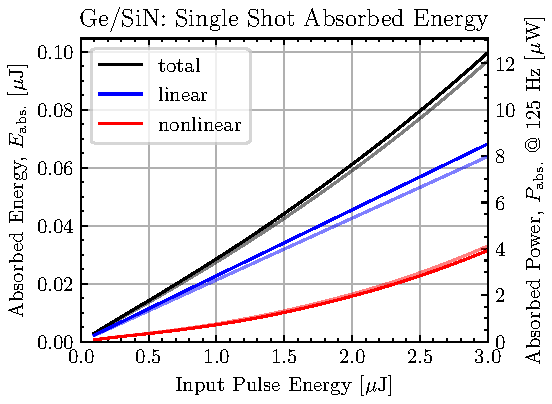
\includegraphics[width=0.75\textwidth]{figures/chap4/Single_shot_abs_ener.pdf}
	\caption{Calculated absorbed energy from a single $\tau_p = 60 \ \textrm{fs}$ pulse at $\lambda=1430 \ \textrm{nm}$ (dark lines) and $\lambda = 1450 \ \textrm{nm}$ (faint lines).}
	\label{fig:Single_shot_abs_ener}
	% python file: \Python Scripts\DrakeIonization\VolumeAveraging_class_script.py
\end{figure}

\cref{fig:Single_shot_abs_ener} plots the absorbed energy and average power for our experimental conditions. The total absorption is calculated using \cref{eqn:absorbed_energy,eqn:absorbed_power}, the linear contribution is calculated using the TMM-predicted effective absorption coefficient of the bilayer $A (1430 \ \textrm{nm}) = 0.023$, and the nonlinear component is the difference between the total and the linear component. We see that the nonlinear absorption is responsible for a little less than half the energy transferred into the sample. For an input pulse energy of 2.75 $\mu$J, only about 0.1 $\mu$J is absorbed by the sample.

\begin{figure}
	\centering
	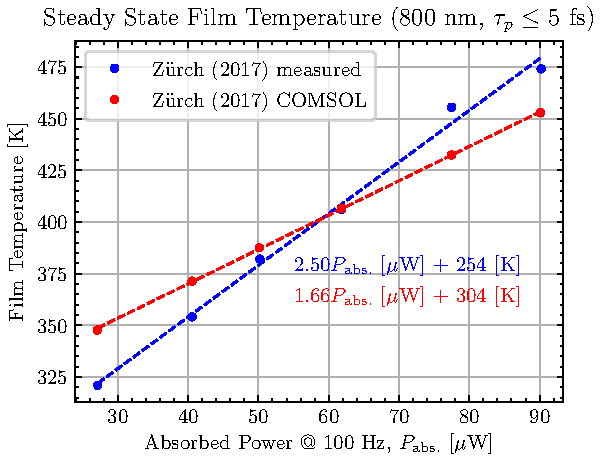
\includegraphics[width=0.75\textwidth]{figures/chap4/COMSOL_temp_power.pdf}
	\caption{Thermal data for a 100 nm Ge/ 30 nm SiN heterostructure extracted from the literature \cite{zurchDirectSimultaneousObservation2017}. \textbf{not sure if this is a valid comparison ... the Zurch spot size is 100 micron vs our 34 micron. the heat distribution will be different.}}
	\label{fig:COMSOL_temp_power}
	% python file: \Python Scripts\DrakeIonization\VolumeAveraging_class_script.py
\end{figure}

The literature reports two estimates of the thin film temperature for a freestanding Ge/SiN membrane with the same geometry as our sample \cite{zurchDirectSimultaneousObservation2017}. In this experiment, they use a $\lambda=760 \ \textrm{nm}$ $\le5 \ \textrm{fs}$ pulse at a 100 Hz repetition rate and an IR FWHM diameter of about 100 $\mu$m to excite the sample. At their interaction intensities, nonlinear effects are negligible, but the absorption coefficient ($A (760 \ \textrm{nm}) = 0.23$) is about 10x higher than at our mid-IR wavelengths. It is reported that sample annealing occurs above 500 K, resulting in permanent sample damage and ultimately limiting the maximum input pulse energy and excitation fraction. \cref{fig:COMSOL_temp_power} shows these two estimates as a function of absorbed power. The first estimate of sample temperature uses a finite element numerical simulation (COMSOL) that takes into account linear absorption by the laser, three dimensional heat diffusion and radiation losses. The second method fits the temperature using the measured indirect bandgap shift to the empirical formula \cite{vinaTemperatureDependenceDielectric1984}:
\begin{equation}
\Delta E_{\textrm{ind.}} = a - \frac{\alpha T^2}{\beta + T},
\label{eqn:CB_shift_temp}
\end{equation}
with $a = 0.741$ eV, $\alpha=4.561 \times 10^{-4}$ eV K$^{-1}$, and $\beta = 210$ K. Both methods yield a linear increase in sample temperature with average absorbed power. The difference between the two estimates is ascribed to an erroneous heat conductivity value used in the COMSOL calculation.

We extrapolate the aforementioned linear fits to estimate our maximum sample temperature. For an absorbed power of 14 $\mu$W, we get a film temperature of $T = 289 \ \textrm{K}$ using the CB shift estimate, and $T = 327 \ \textrm{K}$ using the COMSOL estimate. Both temperature are well below the annealing temperature of 500 K. Taking the higher of the two temperatures, \cref{eqn:CB_shift_temp} predicts $\Delta E_{\textrm{ind.}} = 0.65 \ \textrm{eV}$, which is 20 meV lower than the 0.67 eV value used in \cref{tab:Keldysh_parameters}.


\section{Optimizing experimental ATAS parameters for Germanium thin films}

\subsection{rep rate (avoiding ms-scale excitation)}

\begin{figure}
	\centering
	\subfloat[$\tau \approx 0$ fs, PE = $1.03 \text{ } \mu \text{J}$.]{
		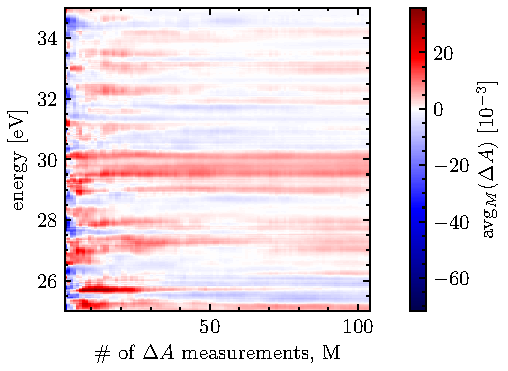
\includegraphics[width=0.4\textwidth]{figures/chap4/StaticOD_1kHz_overlap_1p03uJ.pdf}
		\label{fig:1kHz_Ge_ATAS:overlap_1.03uJ}}
	\qquad
	\subfloat[$\tau \approx 0$ fs, PE = $1.43 \text{ } \mu \text{J}$.]{
		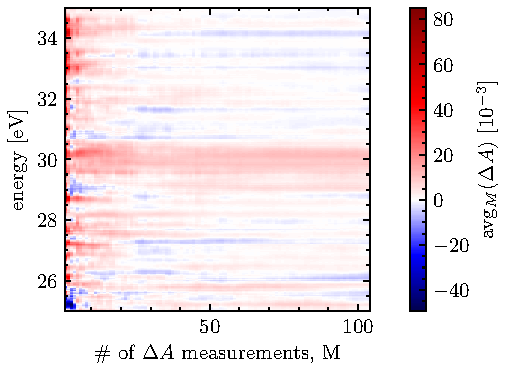
\includegraphics[width=0.4\textwidth]{figures/chap4/StaticOD_1kHz_overlap_1p43uJ.pdf}
		\label{fig:1kHz_Ge_ATAS:overlap_1.43uJ}}
	
	\subfloat[$\tau = - \infty$, PE = $1.03 \text{ } \mu \text{J}$.]{
		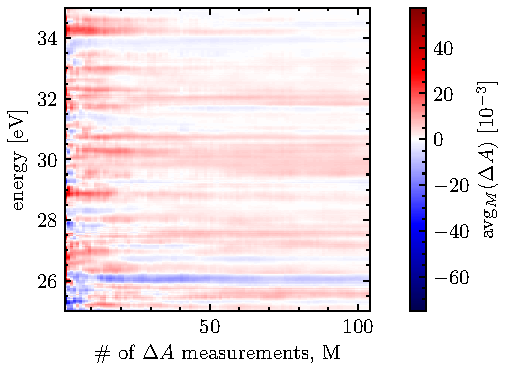
\includegraphics[width=0.4\textwidth]{figures/chap4/StaticOD_1kHz_NegInf_1p03uJ.pdf}
		\label{fig:1kHz_Ge_ATAS:NegInf_1.03uJ}}
	\qquad
	\subfloat[$\tau = - \infty$, PE = $1.43 \text{ } \mu \text{J}$.]{
		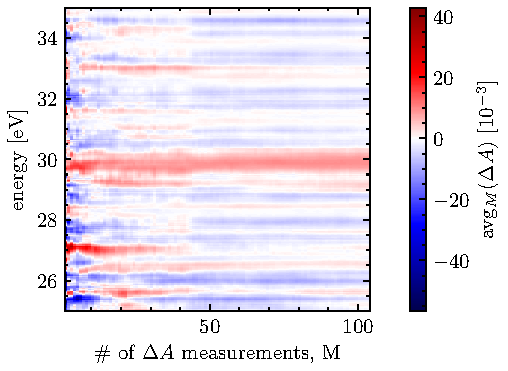
\includegraphics[width=0.4\textwidth]{figures/chap4/StaticOD_1kHz_NegInf_1p43uJ.pdf}
		\label{fig:1kHz_Ge_ATAS:NegInf_1.43uJ}}
	
	\subfloat[PE = $1.03 \text{ } \mu \text{J}$.]{
		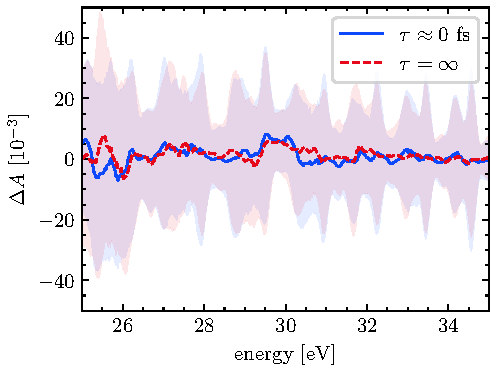
\includegraphics[width=0.4\textwidth]{figures/chap4/StaticOD_avg_1kHz_1p03uJ.pdf}
		\label{fig:1kHz_Ge_ATAS:avg_1.03uJ}}
	\qquad
	\subfloat[PE = $1.43 \text{ } \mu \text{J}$.]{
		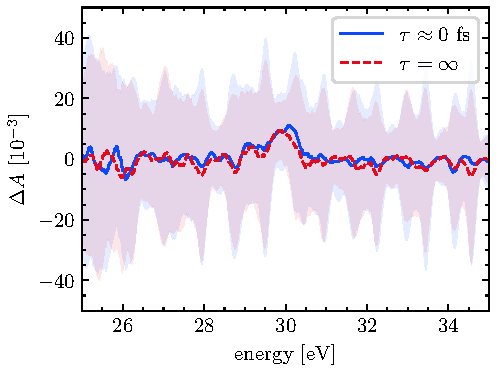
\includegraphics[width=0.4\textwidth]{figures/chap4/StaticOD_avg_1kHz_1p43uJ.pdf}
		\label{fig:1kHz_Ge_ATAS:avg_1.43uJ}}
	\caption{1 kHz fixed-delay ATAS measurements on 100 nm Ge using a $\lambda = 1450 \text{ nm}$ excitation pulse. See text for details.}
	\label{fig:1kHz_Ge_ATAS}
	% datasets: \testdata\2019_08_06\{Avg1,Avg3,Avg4,Avg5}
	% python script: \Python Scripts\Spectrometer\test\2019_08_06.py
\end{figure}

\begin{figure}
	\centering
	\subfloat[$\tau \approx 0$ fs, PE = $1.75 \text{ } \mu \text{J}$.]{
		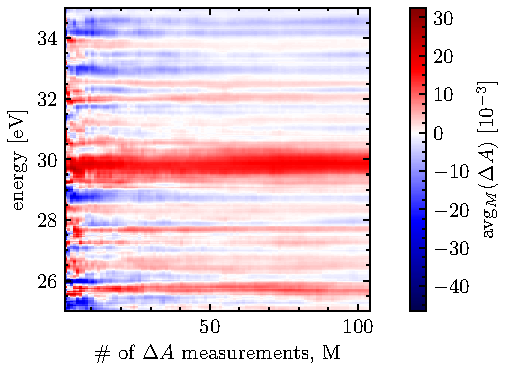
\includegraphics[width=0.4\textwidth]{figures/chap4/StaticOD_1kHz_overlap_1p75uJ.pdf}
		\label{fig:1kHz_Ge_ATAS:overlap_1.75uJ}}
	\qquad
	\subfloat[PE scaling at $\tau \approx 0$ fs.]{
		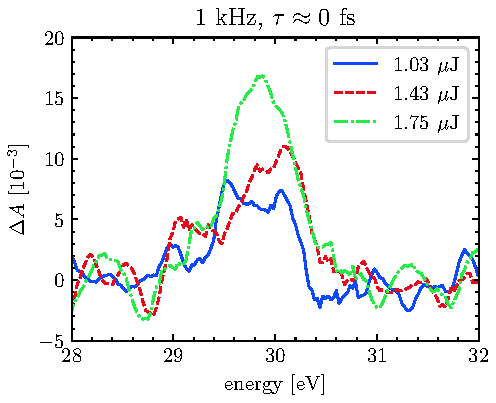
\includegraphics[width=0.4\textwidth]{figures/chap4/StaticOD_avg_1kHz_PE_scaling.pdf}
		\label{fig:1kHz_Ge_ATAS:PE_scaling}}
	
	\subfloat[PE = $1.43 \text{ } \mu \text{J}$.]{
		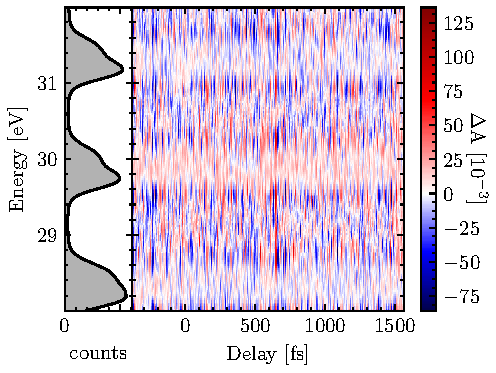
\includegraphics[width=0.4\textwidth]{figures/chap4/ODvsDelay_1kHz_1p43uJ.pdf}
		\label{fig:1kHz_Ge_ATAS:delay_1.43uJ}}
	\qquad
	\subfloat[PE = $1.75 \text{ } \mu \text{J}$.]{
		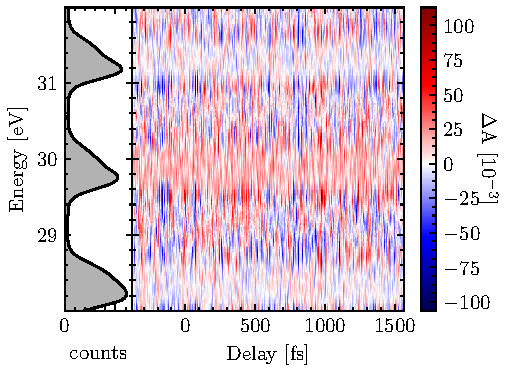
\includegraphics[width=0.4\textwidth]{figures/chap4/ODvsDelay_1kHz_1p75uJ.pdf}
		\label{fig:1kHz_Ge_ATAS:delay_1.75uJ}}
	
	\subfloat[PE = $1.43 \text{ } \mu \text{J}$ (rolling average).]{
		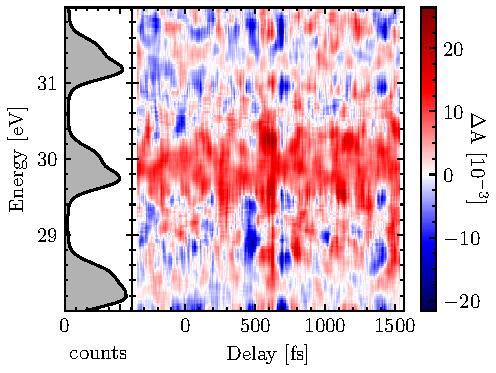
\includegraphics[width=0.4\textwidth]{figures/chap4/ODvsDelay_20roll_1kHz_1p43uJ.pdf}
		\label{fig:1kHz_Ge_ATAS:roll_delay_1.43uJ}}
	\qquad
	\subfloat[PE = $1.75 \text{ } \mu \text{J}$ (rolling average).]{
		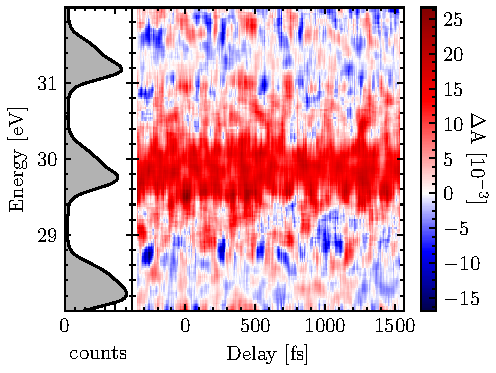
\includegraphics[width=0.4\textwidth]{figures/chap4/ODvsDelay_20roll_1kHz_1p75uJ.pdf}
		\label{fig:1kHz_Ge_ATAS:roll_delay_1.75uJ}}
	\caption{1 kHz ATAS measurements in Ge using a $\lambda = 1450 \text{ nm}$ excitation pulse. \cref{fig:1kHz_Ge_ATAS:overlap_1.75uJ}: fixed-delay ATAS measurements with a pulse energy of 1.75 $\mu$J. \cref{fig:1kHz_Ge_ATAS:PE_scaling}: Pulse energy scaling at overlap of 1 kHz measurements. \cref{fig:1kHz_Ge_ATAS:delay_1.43uJ,fig:1kHz_Ge_ATAS:delay_1.75uJ,fig:1kHz_Ge_ATAS:roll_delay_1.43uJ,fig:1kHz_Ge_ATAS:roll_delay_1.75uJ}: delay scans at 1 kHz.  \cref{fig:1kHz_Ge_ATAS:delay_1.43uJ,fig:1kHz_Ge_ATAS:delay_1.75uJ}: raw delay scan data. \cref{fig:1kHz_Ge_ATAS:roll_delay_1.43uJ,fig:1kHz_Ge_ATAS:roll_delay_1.75uJ}: rolling average of the raw data with a 65 fs window (20 delay points). The left panel on each spectrogram shows the ground state spectrum $S_{gs}(E)$. See text for details.}
	\label{fig:1kHz_Ge_ATAS:delay}
	% datasets: \testdata\2019_08_06\{Delay1,Delay2}
	% python script: \Python Scripts\Spectrometer\test\2019_08_06.py
\end{figure}

\begin{figure}
	\centering
	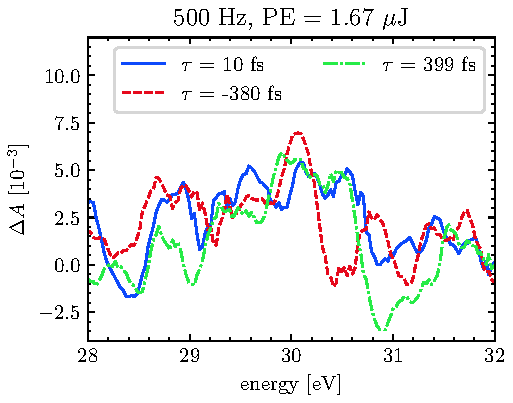
\includegraphics[width=0.75\textwidth]{figures/chap4/StaticOD_avg_500Hz_1p67uJ.pdf}
	\caption{500 Hz ATAS measurements in Ge using a $\lambda = 1450$ nm, 1.67 $\mu$J excitation pulse. Each delay curve is an average of 104 identical measurements. The sample shows no delay dependance within the uncertainty of the measurement.}
	\label{fig:500Hz_Ge_ATAS:delays}
	% dataset: C:\testdata\2019_08_06\HWP1{Avg8,Avg9,Avg10}
	% python file: \Python Scripts\Spectrometer\test\2019_08_06.py
\end{figure}

\begin{figure}
	\centering
	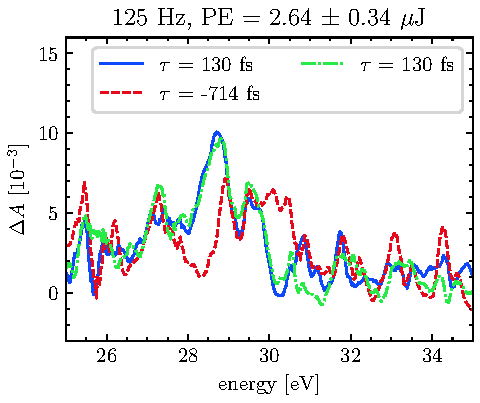
\includegraphics[width=0.75\textwidth]{figures/chap4/StaticOD_avg_125Hz_2p64uJ.pdf}
	\caption{125 Hz ATAS measurements in Ge using a $\lambda = 1450$ nm, 2.64 $\mu$J excitation pulse. Each lineout represents the average of 394 measurements. See text for details.}
	\label{fig:125Hz_Ge_ATAS:static_delays}
	% dataset: C:\testdata\2019_08_13\Avg1,2,3
	% python file: Python Scripts\Spectrometer\test\2019_08_13.py
\end{figure}

\begin{figure}
	\centering
	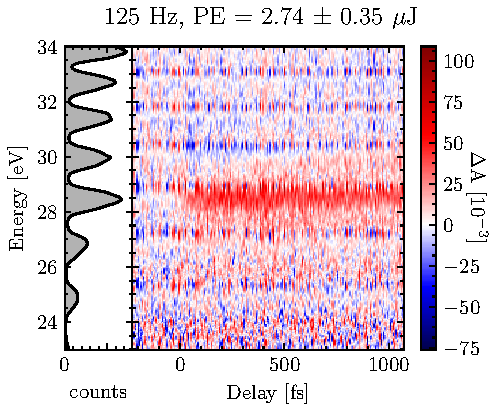
\includegraphics[width=0.75\textwidth]{figures/chap4/Delay234_1450nm_125HzuJ.pdf}
	\caption{125 Hz delay scan in Ge using a $\lambda = 1450$ nm, 2.74 $\pm$ 0.35 $\mu$J excitation pulse. This is an average of 3 repeated measurements. See text for details.}
	\label{fig:125Hz_Ge_ATAS:delay_scan}
	% dataset: C:\testdata\2019_08_13\Delay2,3,4 averaged together.
	% python file: Python Scripts\Spectrometer\test\2019_08_13.py
\end{figure}

We performed exploratory experiments at 1 kHz to determine the optimal excitation pulse energy. For this set of measurements, we generated harmonics in Argon using $\lambda$ = 1450 nm, a 200 nm Al filter and the $2C$ optics removed (see \cref{fig:beamline_schematic}). Two delay points were recorded: with the XUV and IR pulses overlapped ($\tau = 0$) and with the XUV pulse arriving about 300 fs before the IR ($\tau = -\infty$). For each delay point, we used three pulse energies: 1.03, 1.43 and 1.75 $\mu$J. To increase the signal-to-noise, we performed each experiment 104 times and averaged the datasets. The exposure time was 0.5 seconds, and the sample was rastered so that each measurement was recorded at a new position on the sample. The results are shown \cref{fig:1kHz_Ge_ATAS,fig:1kHz_Ge_ATAS:overlap_1.75uJ,fig:1kHz_Ge_ATAS:PE_scaling}. 

\cref{fig:1kHz_Ge_ATAS:overlap_1.03uJ,fig:1kHz_Ge_ATAS:overlap_1.43uJ,fig:1kHz_Ge_ATAS:NegInf_1.03uJ,fig:1kHz_Ge_ATAS:NegInf_1.43uJ,fig:1kHz_Ge_ATAS:overlap_1.75uJ} show the average $\Delta A$ as a function of the number of averaged measurements, $M$. Spectral features are apparent after averaging about 10 datasets together, but the fidelity of the signal does not appreciably improve after the first $M=50$ datasets. \cref{fig:1kHz_Ge_ATAS:avg_1.03uJ,fig:1kHz_Ge_ATAS:avg_1.43uJ} show the average signal (lines) and the standard deviation (shaded area), as calculated from the entire ensemble of measurements. The data is noisy, but we can see a spectral feature near 30 eV which scales with pulse energy (or perhaps average power). This behavior is evident in \cref{fig:1kHz_Ge_ATAS:PE_scaling}. However, this feature is delay-independent: $\Delta A$ has nearly the same value regardless of whether the XUV arrives before or after the IR pulse.

To confirm the delay-independence of this feature, we performed delay scans at two different pulse energies (1.43 and 1.75 $\mu$J). These measurements are shown in \cref{fig:1kHz_Ge_ATAS:delay}. Delay was controlled by inserting a fused silica wedge into the inteferometer (W in \cref{fig:beamline_schematic}). Each delay step corresponds to approximately 3.25 fs (25 $\mu$m of wedge insertion).

The raw data is shown in \cref{fig:1kHz_Ge_ATAS:delay_1.43uJ,fig:1kHz_Ge_ATAS:delay_1.75uJ}. As this experiment was only performed once ($M=1$), the contrast is poor and the 30 eV feature is barely visible. The spectral feature becomes more prominent after performing a rolling average over 20 delay points (65 fs), which is shown in \cref{fig:1kHz_Ge_ATAS:roll_delay_1.43uJ,fig:1kHz_Ge_ATAS:roll_delay_1.75uJ}. These delay measurements confirm our suspiscion that the absorption feature is delay-independent at 1 kHz.

One possible origin of a delay-independent signal can be a very long-lived excited state with lifetime $1/\Gamma$. Each laser shot initiates an assortment of electron and phonon dynamics, each with their own time scales. If any of these excited states have time scales that approach the inverse rep. rate of the laser ($1/RR$), then the dynamics from the previous shot will still be evolving by time the next shot arrives. Since each exposure integrates over hundreds or thousands of laser shots, measurements at a nomimal delay $\tau$ will contain information from several delays $\tau_i$, each separated by the time between laser shots: $\tau_i = \tau, \tau-\frac{1}{RR}, \tau-\frac{2}{RR}, \dots$, with the amplitude of each contribution weighed by an exponential decay factor $\exp(+ \tau_i \Gamma)$. If this is the case, then the magnitude of the delay-independent signal should decrease as time between laser shots is increased. As the time between laser shots is increased past the lifetime of the state, the excited state population from the previous laser shot will be small enough to observe the dynamics of the shorter-lived states. Experimentally, we can accomplish this by adjusting the rep. rate divider on the Spitfire amplifier (which reduces the rep. rate), and/or using an optical chopper.

The rep. rate was halved to 500 Hz using the Spitfire's rep. rate divider ($m=2$) and the exposure time was doubled to 1 second so that the number of laser shots per exposure was held constant. A series of fixed-delay measurements were recorded using a 1.67 $\mu$J pulse energy, shown in \cref{fig:500Hz_Ge_ATAS:delays}. The spectral feature at 30 eV is still present, but it does not exhibit any delay dependence within the uncertainty of the measurement. It is notable that, for a similar pulse energy, the magnitude of the feature at 500 Hz is half that of the 1 kHz measurement. This is consistent with the hypothesis of a long-lived state contributing to the signal.

The rep. rate was lowered to 125 Hz using a combination of the rep. rate divider ($m=4$) and an optical chopper ($T = 50\%$) placed after the TOPAS. The exposure time was increased to 4 seconds to maintain sufficient counts on the detector. An ATAS spectrum was recorded about 130 fs after temporal overlap and several hundred fs before overlap using a 2.64 $\pm$ 0.34 $\mu$J excitation pulse ($\lambda$ = 1450 nm), as shown in \cref{fig:125Hz_Ge_ATAS:static_delays}. A second measurement after overlap was recorded to ensure repeatability. At negative delays (red curve), we see the familiar 30 eV feature, albeit weaker at $6 \times 10^{-3}$. Near overlap, we see a new feature emerge at 28.7 eV, with a magnitude of $\approx 10 \times 10^{-3}$. This observation is consistent with long-lived excited state at 30 eV. A delay scan at 125 Hz, shown in \cref{fig:125Hz_Ge_ATAS:delay_scan}, reveals that the 28.7 eV feature is indeed time-dependent with a ps-scale lifetime.


\subsection{IR pulse energy}

\subsection{harmonic spectrum ($\lambda$, 2-color generation)}

\begin{figure}
	\centering
	\subfloat[125 Hz ($M=6$)]{
		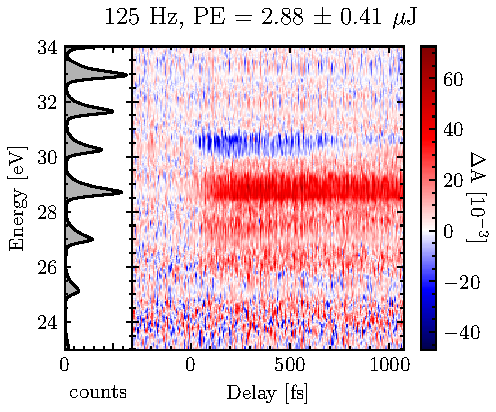
\includegraphics[width=0.4\textwidth]{figures/chap4/Delay123456_1430nm_125Hz_2p88uJ.pdf}
		\label{fig:125Hz_1430nm_Ge_ATAS:delay123456}}
	\qquad
	\subfloat[250 Hz ($M=2$)]{
		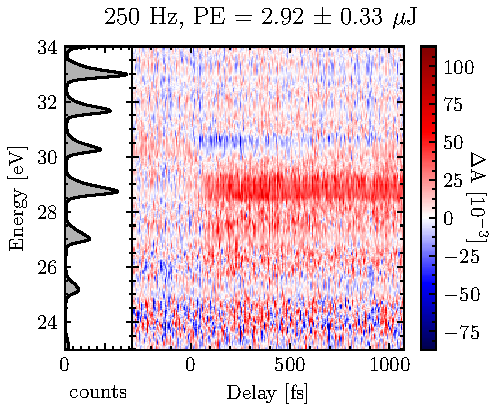
\includegraphics[width=0.4\textwidth]{figures/chap4/Delay89_1430nm_250Hz_2p92uJ.pdf}
		\label{fig:250Hz_1430nm_Ge_ATAS:delay89}}
	
	\caption{125 vs. 250 Hz measurements at $\lambda$ = 1430 nm. }
	\label{fig:125vs250Hz_1430nm_Ge_ATAS:delay}
	% datasets:
	% 125 Hz: \testdata\2019_08_15\125Hz\Delay1-6 averaged
	% 250 Hz: \testdata\2019_08_15\250Hz\Delay8,9 averaged
	% python script: \Python Scripts\Spectrometer\test\2019_08_15.py
\end{figure}

The fundamental wavelength was decreased by 20 nm to 1430 nm, where the absorption length in Ge is about 5\% shorter. For a fixed pulse energy, this increases the excitation fraction and thus the strength of the $\Delta A$ signal. Changing the wavelength also changes which initial and final states near the Fermi level are populated, according to the band structure calculations in \cref{fig:Ge_band_diagram}. Using this shorter wavelength we can observe a more robust sample response, as shown in \cref{fig:125vs250Hz_1430nm_Ge_ATAS:delay}.

At 1430 nm, we can see a sample response from 25.7 to 31 eV. From 25.7 to 30 eV, there is a broad increase in absorption, with the largest increase occuring between 28.4 and 29.5 eV. A decrease in absorption occurs between 30 and 31 eV. These features are present in both the 125 and 250 Hz data. The 30 eV negative delay feature persists in the 250 Hz dataset, but at $12 \times 10^{-3}$ it does not overwhelm the rest of the sample response. Further measurements were performed at either 125 Hz to suppress the static feature, or at 250 Hz to minimize data collection time.


\subsection{optimized ATAS Ge experimental results}

\subsection{post-experiment analysis: verify we didn't permanently damage sample}

\section{Data Analysis}

\subsection{description of data pipeline}
\subsubsection{going from 2D image to 1D spectra}

\begin{figure}
	\centering
	\includegraphics[width=0.75\textwidth]{figures/chap4/data_pipeline.png}
	\caption{this cartoon shows the data pipeline. it is an overview of all the processing steps i do on the data.}
	\label{fig:data_pipeline}
	% dataset: ???
	% python file: ???
\end{figure}

background subtraction, selecting a divergence window, normalization by exposure time \& divergence window, integration over divergence window




\subsubsection{$A$, $\Delta A$ calculation}

\subsection{systematic noise sources in our experiment}

\subsection{methods to numerically correct for harmonic noise and drift}

\subsection{frequency filtering to remove $\omega, 2 \omega$ oscillations}

\section{Physical Interpretation of spectra}
\subsection{decomposition of spectral response}
\subsection{description of observed dynamics}